\documentclass{article}

\pagenumbering{gobble}

\usepackage{graphicx}
\usepackage[square,numbers]{natbib}
\renewcommand{\bibname}{References}
\usepackage{xcolor}
\usepackage{enumitem}
\usepackage{bigfoot}
\usepackage{pdfpages}
\usepackage{hyperref}
\hypersetup{
    colorlinks,
    linkcolor={black},
    citecolor={blue!35!black},
    urlcolor={blue!35!black}
}

\usepackage[bottom]{footmisc}
\usepackage[nottoc]{tocbibind}
\usepackage{amsmath}
\usepackage[utf8x]{inputenc}
\usepackage{amssymb, upgreek}
\usepackage[toc,page]{appendix}

\usepackage{color}
\definecolor{keywordcolor}{rgb}{0.7, 0.1, 0.1}   % red
\definecolor{commentcolor}{rgb}{0.4, 0.4, 0.4}   % grey
\definecolor{symbolcolor}{rgb}{0.0, 0.1, 0.6}    % blue
\definecolor{sortcolor}{rgb}{0.1, 0.5, 0.1}      % green
\definecolor{errorcolor}{rgb}{1, 0, 0}           % bright red
\definecolor{stringcolor}{rgb}{0.5, 0.3, 0.2}    % brown

\usepackage{listings}
\def\lstlanguagefiles{lstlean}
\lstset{language=lean}

\begin{document}

\section*{Talk: Provable Determinism in Reactors}

This talk is going to be about my bachelor thesis \emph{Provable Determinism in Reactors}, in which I show how to formalize a small
subset of the \emph{Reactor model} using a tool called \emph{Lean}, and
prove that execution of such simplified Reactors is deterministic. Just
for some context: This presentation is actually part of my defense for
this thesis. Since part of it is about motivating Reactors, which
shouldn't be necessary for this audience, I'll be skipping some slides.
So what I want to talk about \emph{today} is mainly Lean, i.e.~the tool
for formalizing Reactors and proving properties about them.

To get started, let's briefly consider what this talk is \emph{not}
going to be about.

\begin{center}
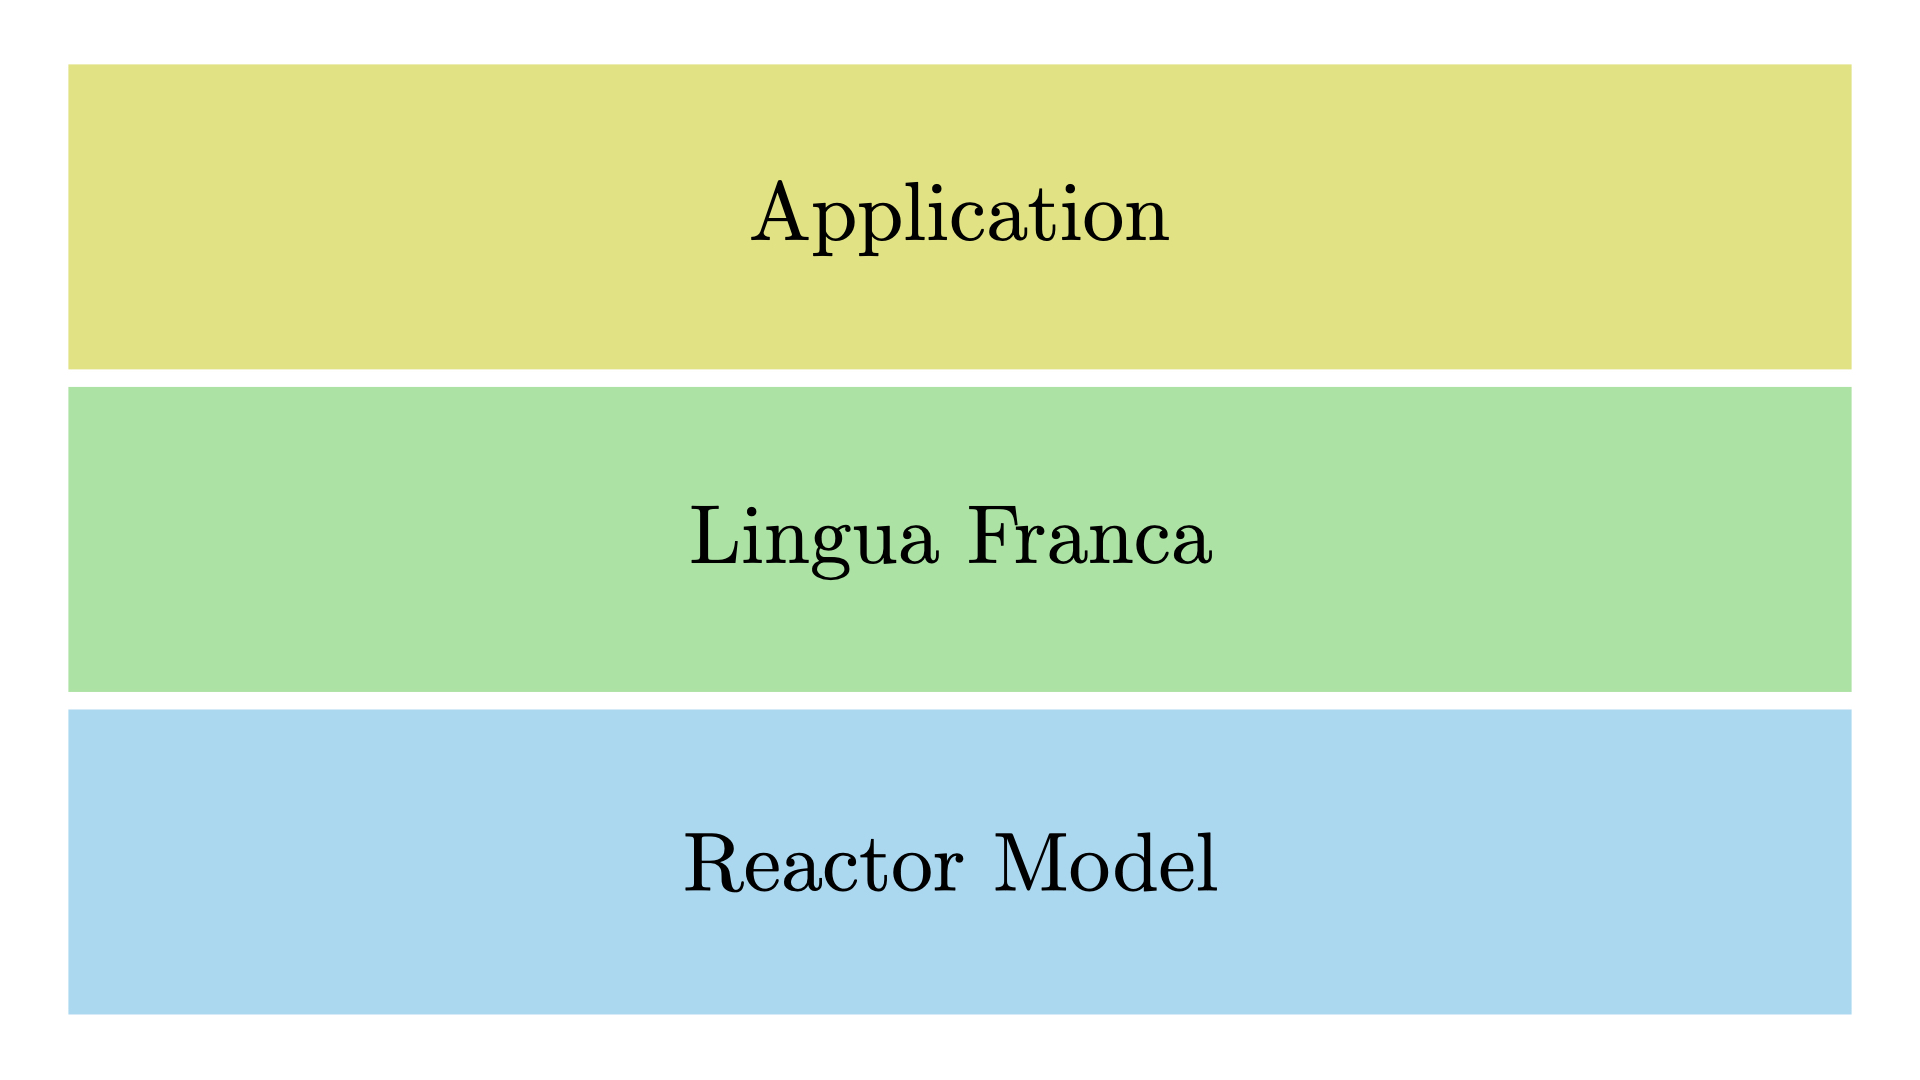
\includegraphics[width=\columnwidth]{Slides/Slide 1.jpeg}
\end{center}

I'm guessing you're all familiar with \emph{Lingua Franca}, which is a
software framework upon which we can build (concurrent) applications.
What we hope to attain by building applications upon this framework, are
certain beneficial properties like loose coupling, testability and
determinism. Lingua Franca adheres to the structure defined in the
Reactor model, which is a purely mathematical description of reactors,
their components and behaviors. One of the reasons we build the software
framework on this mathematical foundation is so that we can actually
\emph{prove} those beneficial properties that we're trying to attain. So
while we're \emph{hoping} that Lingua Franca gives us, for example,
determinism, we can actually \emph{prove} this mathematically for the
Reactor model.

This endeavor raises some meta-problems. First, how can show that Lingua
Franca actually adheres to the Reactor model? Second, how can we be sure
that our mathematical formalization is actually well-defined and our
proofs are valid? We won't tackle the first problem here, but instead
focus on the second one. And the second problem really isn't unique to
the Reactor model, but applies to mathematics as a whole: How can we be
sure that mathematical work is correct?

\begin{center}
  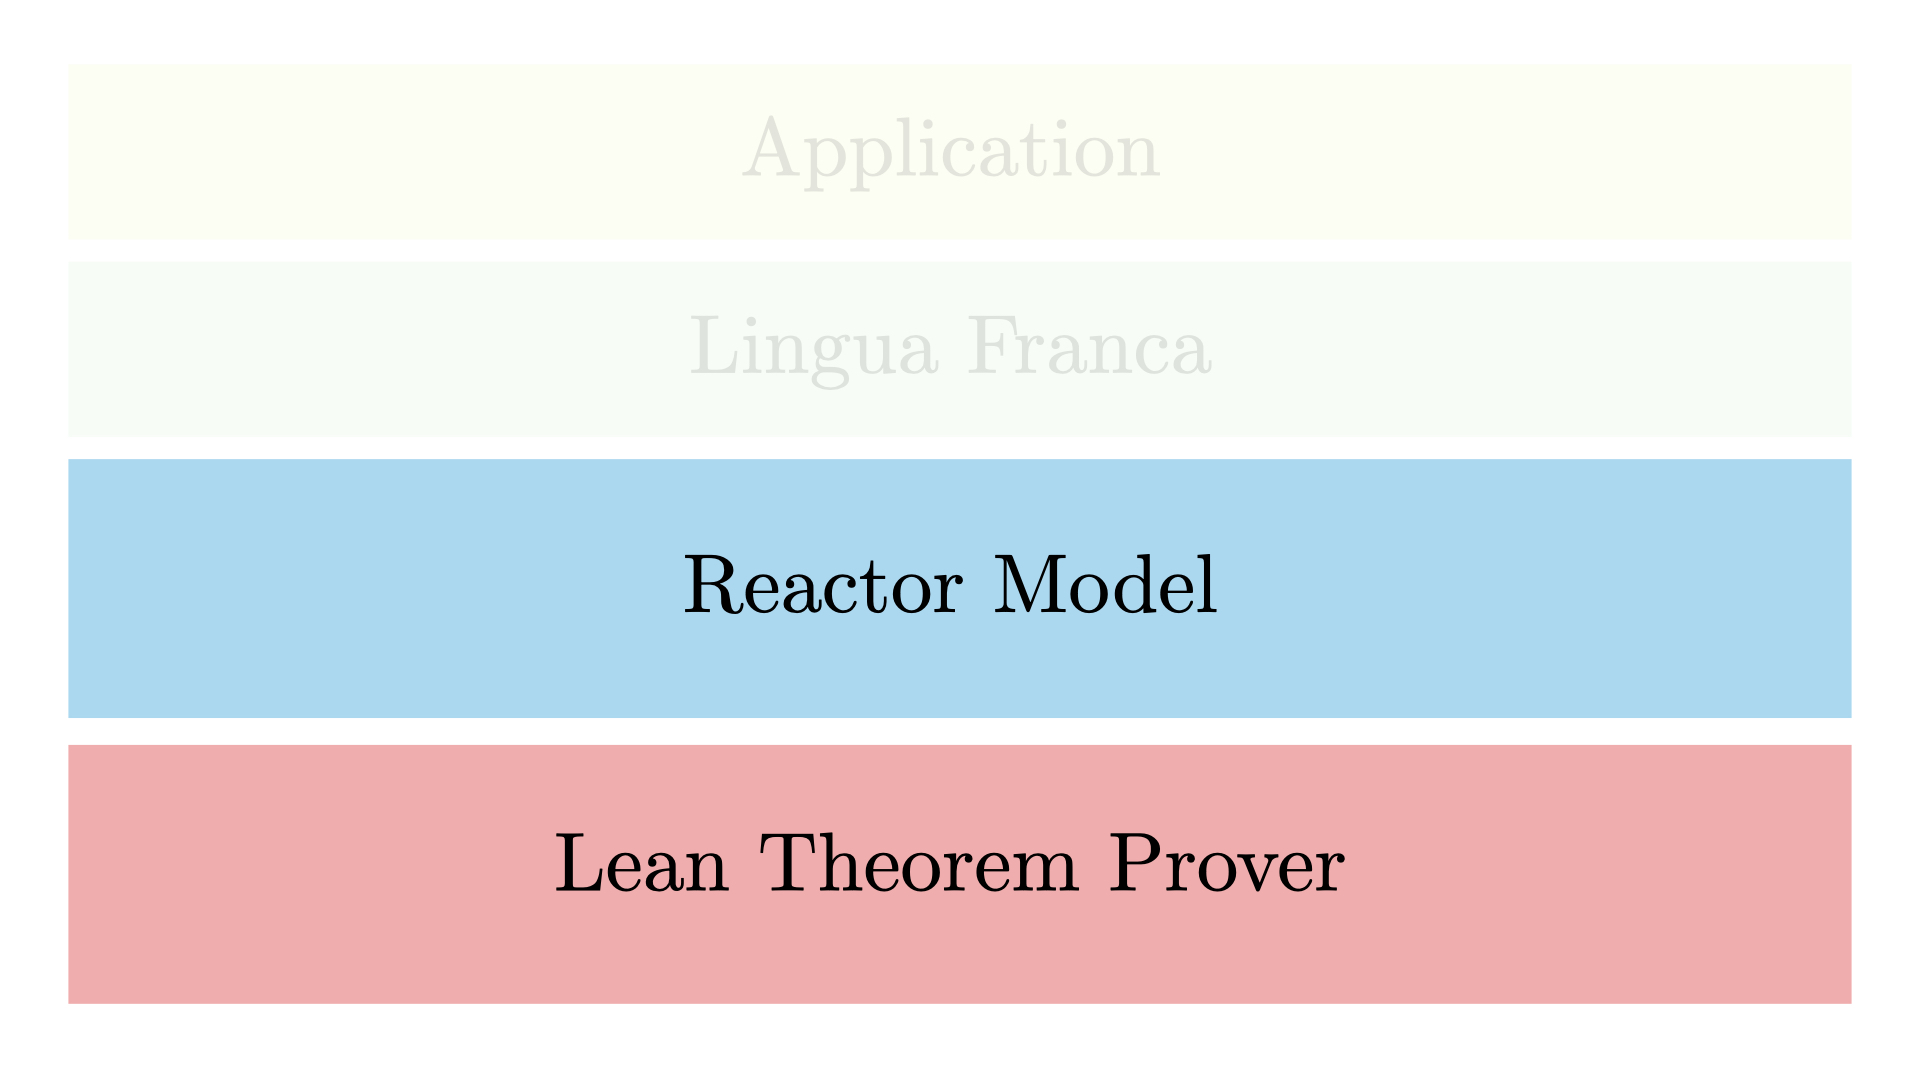
\includegraphics[width=\columnwidth]{Slides/Slide 2.jpeg}
\end{center}

This is where Lean Theorem Prover plays its part. Lean is a tool for
formalizing mathematics, such that we can be (almost) certain that it's
error-free. So what I'd like to show you in the next couple of minutes
are, firstly the foundations of Lean that are necessary for working with
this tool and secondly a hands-on example of formalizing a (very small)
piece of the Reactor model.

\begin{center}
  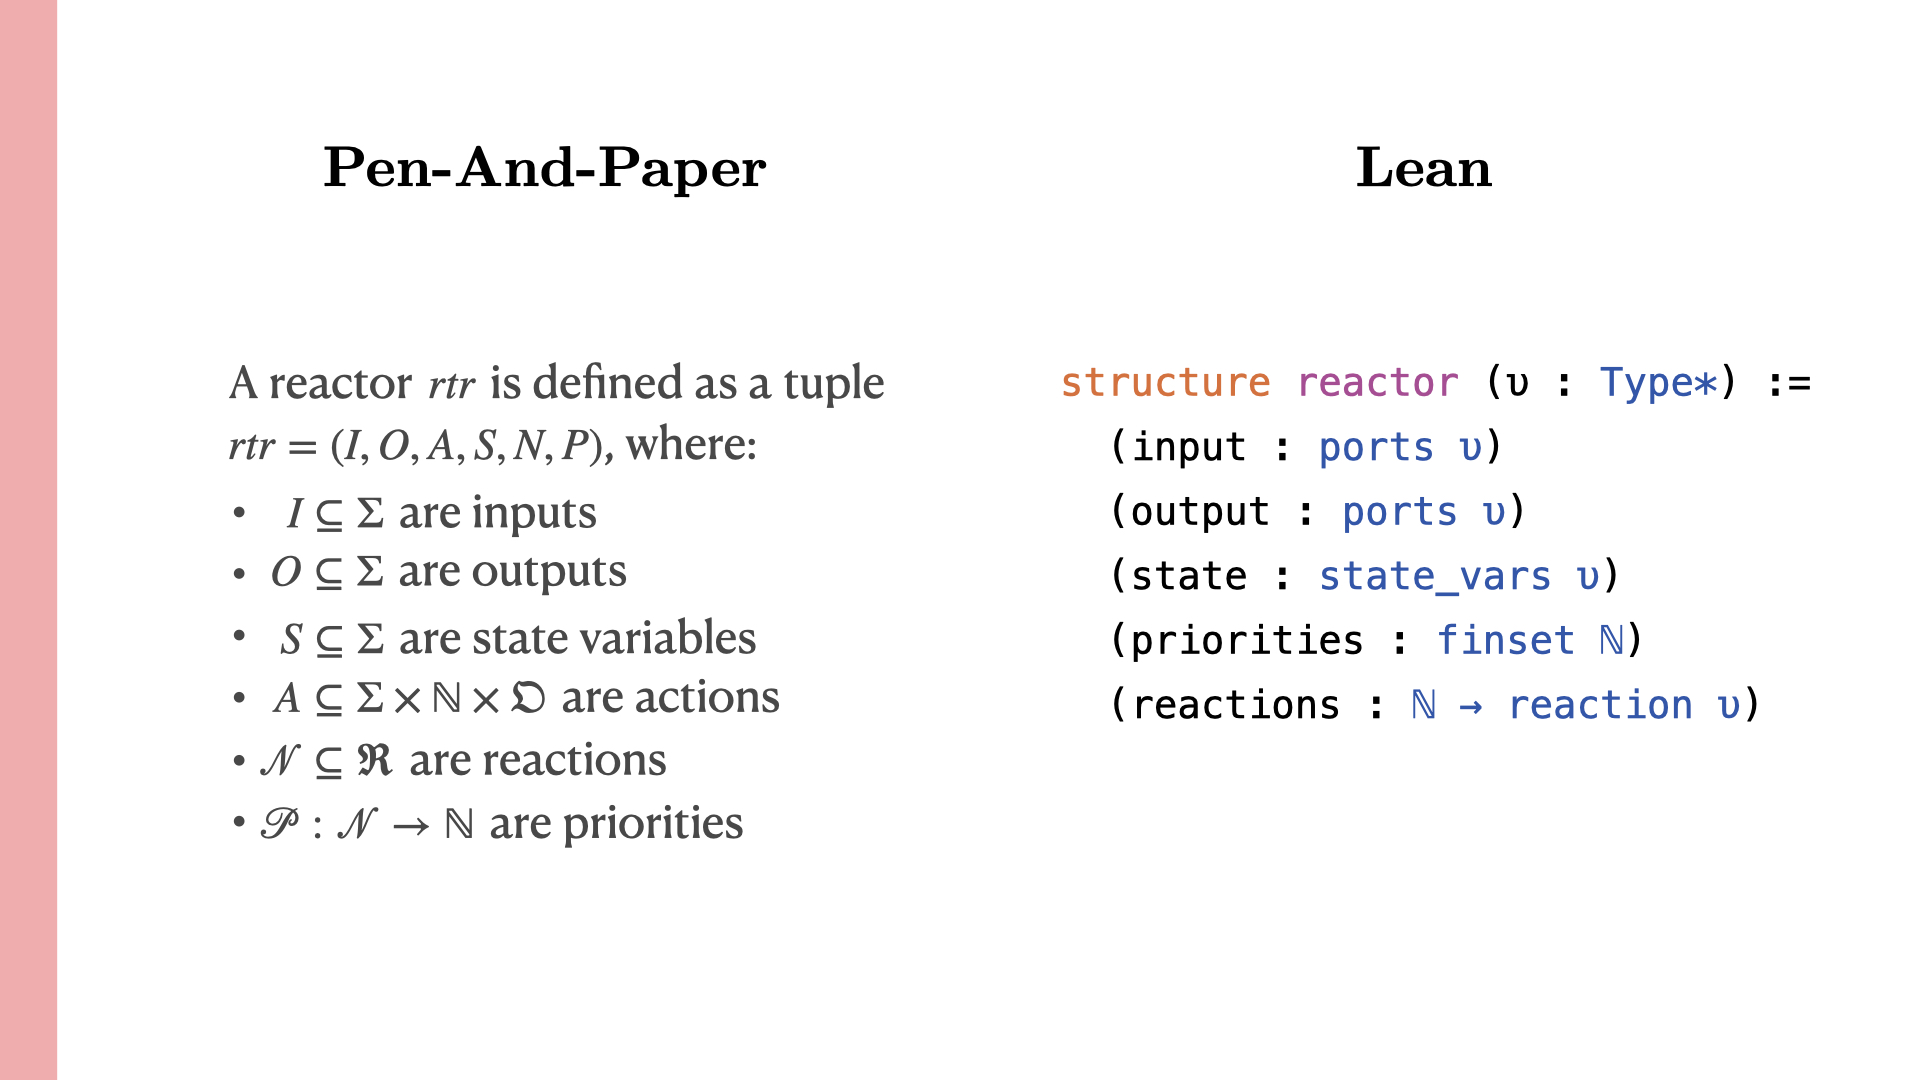
\includegraphics[width=\columnwidth]{Slides/Slide 3.jpeg}
\end{center}

I don't know your backgrounds, but I'm guessing that most of you have
worked with traditional, pen-and-paper mathematical definitions like the
ones shown on the left. For example, here we define what a reactor is,
and notably, we use the language of set theory and predicate logic.
That's the norm in traditional mathematics: we use ZFC set theory (which
is based on predicate logic). On the right side, you can see what
definitions look like in Lean. While this looks a lot like regular
programming language code, in part because of the font and colors, this
is actually a strictly mathematical definition. So in the following
slides, when you see code like this, try to read it as
\emph{mathematical notation} not \emph{programming language code}.

Even though this code snippet is a mathematical definition, there's
actually a fundamental difference relative to the definition on the
left: The mathematical foundations for Lean are not ZFC, but something
called the \emph{Calculus of Inductive Constructions} (CiC). CiC is not
a theory of \emph{sets}, but a theory of \emph{types}. Hence, creating
formalizations in Lean requires us to first (briefly) review these
different mathematical foundations. Luckily, this will also provide us
with an opportunity to introduce some of Lean's syntax.

\begin{center}
  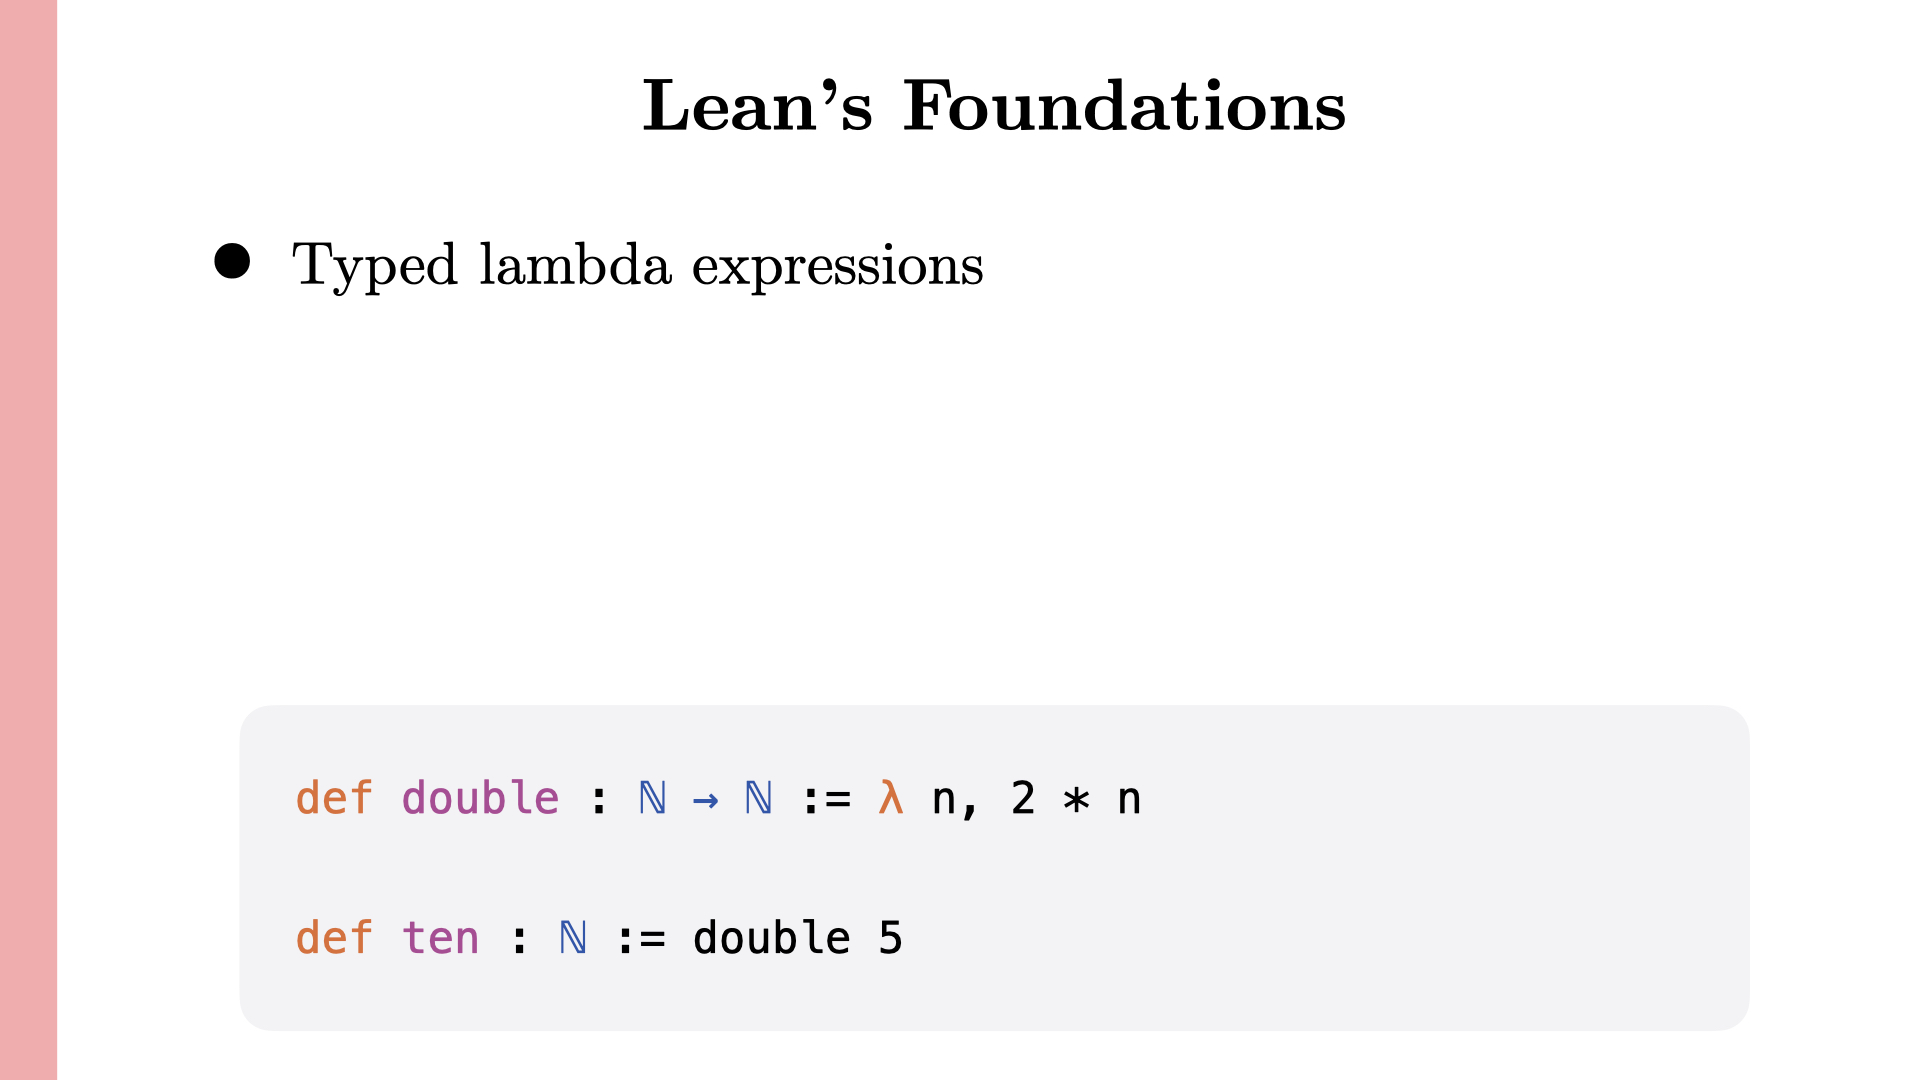
\includegraphics[width=\columnwidth]{Slides/Slide 4.jpeg}
\end{center}

CiC based on \emph{Lambda Calculus}, which most of you probably had to
learn during your studies at some point. If not, it suffices to know
that this is a model of computation (like Turing machines), which
provides us with a concept of \emph{functions} and hence
\emph{computation}. In CiC we use a flavor of lambda calculus, which is
\emph{typed}. That is, every term has an associated type --- just like in
typed programming languages. At bottom of this slide you can see
examples of this (this is valid Lean syntax). First of all, we define a
function called \lstinline{double}, which has the type \lstinline{ℕ → ℕ} and
is defined by the term \lstinline{λ n, 2 * n}, which maps a natural
number \lstinline{n} to the natural number \lstinline{2 * n}. This is an
example of how we can define a function. Secondly, we have an example of
applying a function: The symbol \lstinline{ten} is a natural number,
defined by the result of applying the function \lstinline{double} to the
value \lstinline{5}. These are the basic notions of computation in typed
lambda calculus. And if you've ever programmed in a typed programming
language, these basic type-related notions should come quite natural to
you. But if you tend to make heavy use of types your style of
programming, Lean should be all the more exciting for you, because in
Lean types and values are strongly intermingled. This has to do with the
second fundamental aspect of Lean, called \emph{dependent types}.

\begin{center}
  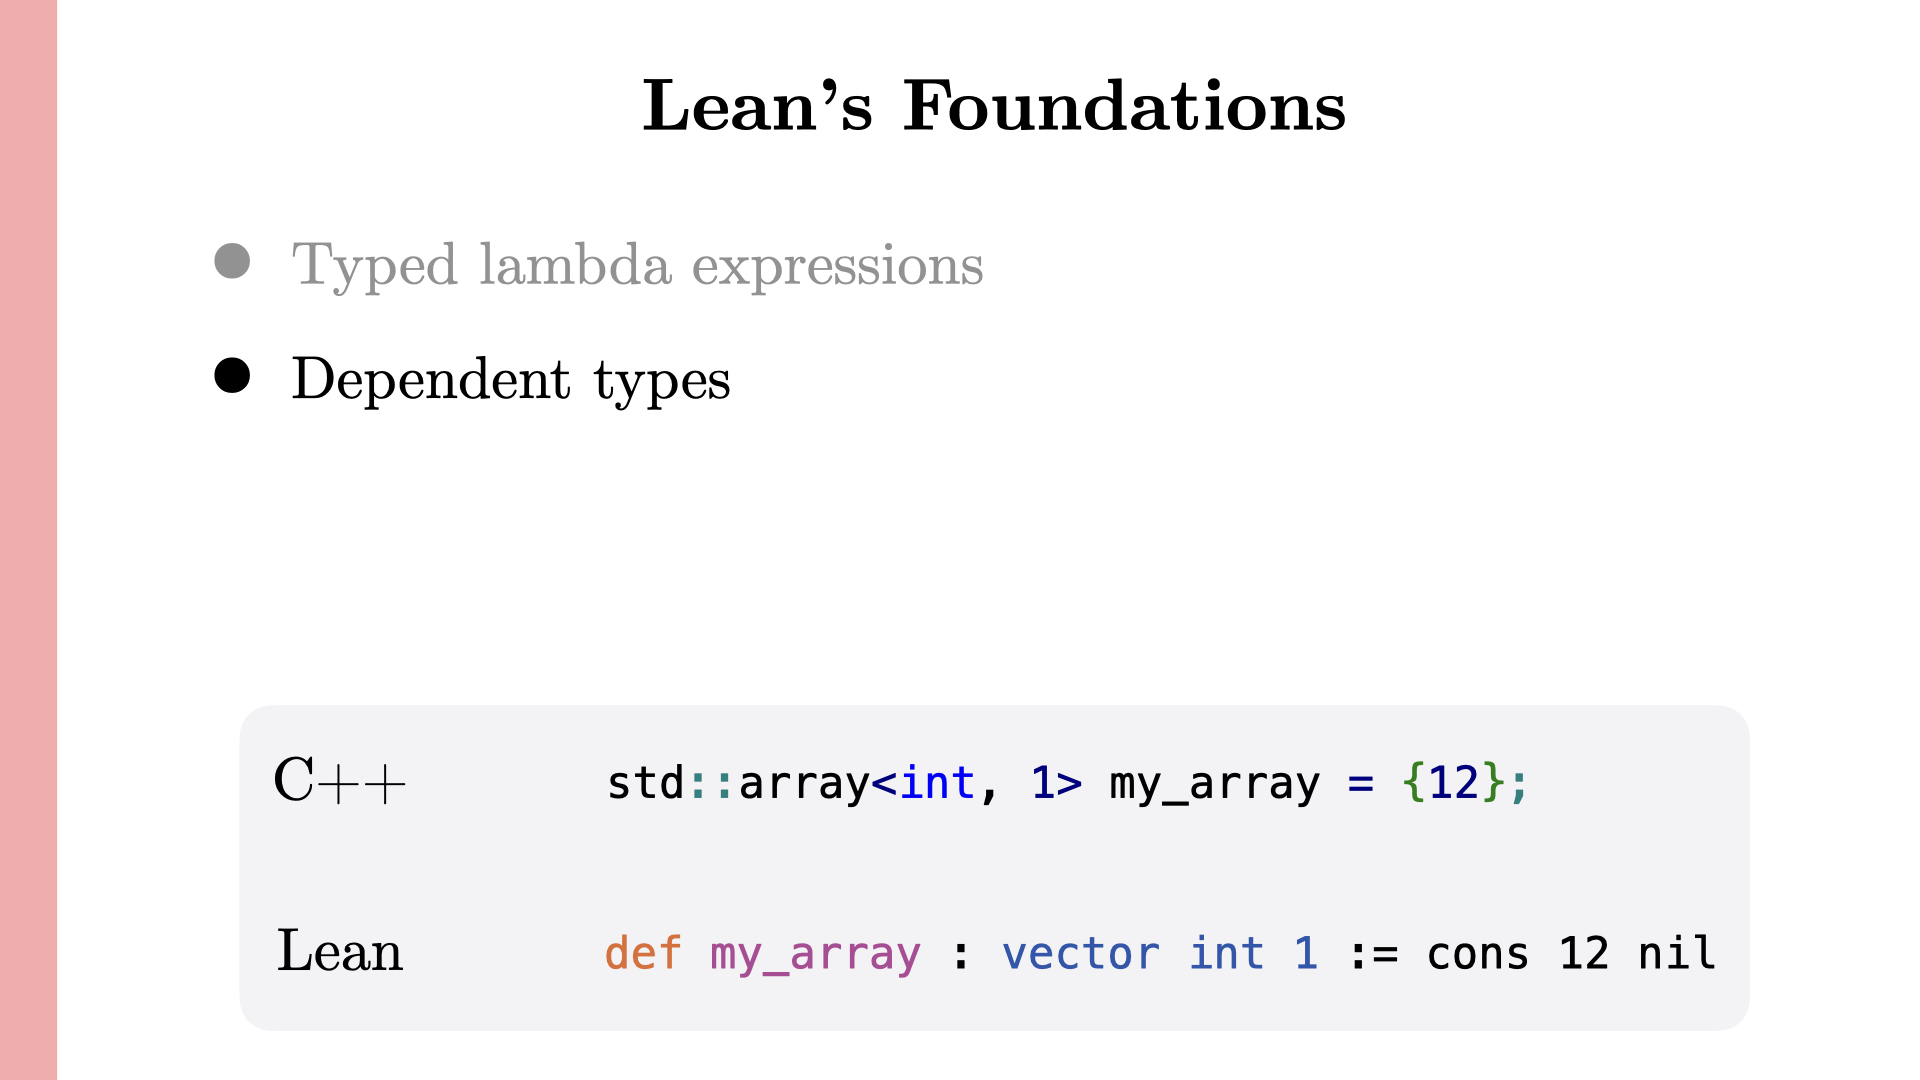
\includegraphics[width=\columnwidth]{Slides/Slide 5.jpeg}
\end{center}

If you've ever written generic code, you might have wished you could add
a value as a generic parameter. E.g. you might want to program an array
type that has a fixed length, without requiring special compiler
support. C++ has \emph{some} support for this, so you can write the code
shown at the bottom. But this only works for statically determined
values. In Lean values can naturally be a part of types, without any
constraints. So we can express precisely the same definition in Lean
using the \lstinline{vector} type. Thus, the type of \lstinline{my_array} is
precisely \lstinline{vector int 1}, making the value \lstinline{1} part of
the type. And in fact, the value doesn't have to be a static \lstinline{1},
but could be the result of some function call. The origin of dependent
types are \emph{dependent functions}, which we can talk about later if
you're interested. So dependent parameters are a neat aspect of types in
Lean, but how do we even define a type - e.g.~how is \lstinline{vector}
defined? To uncover this, we'll have to consider another key aspect of
Lean: \emph{inductive types}. They are the main mechanism by which we
define new types, and by extension values, in Lean. As an example, let's
consider the definition of the \lstinline{list} type (from which the
\lstinline{vector} type is derived).

\begin{center}
  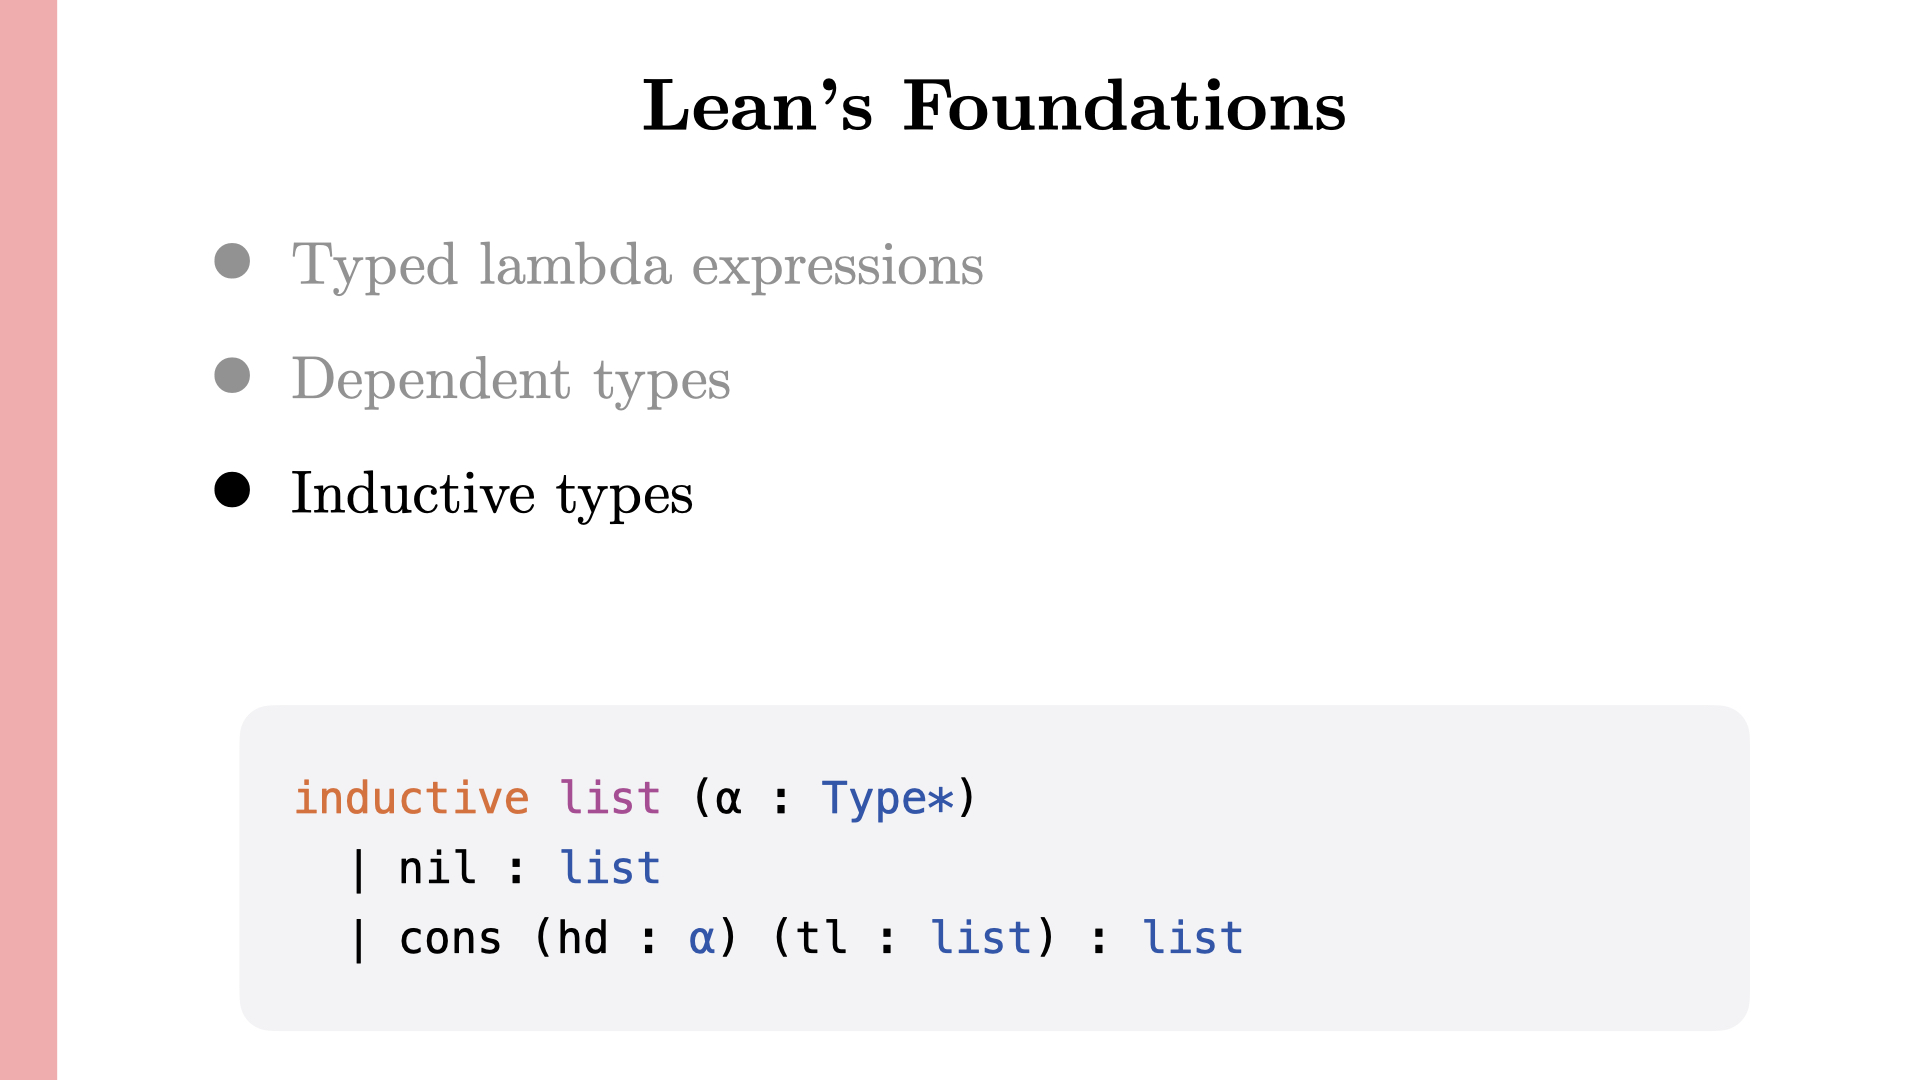
\includegraphics[width=\columnwidth]{Slides/Slide 6.jpeg}
\end{center}

What you see here is an inductive type definition. This is like a scheme
for how to make instances of the \lstinline{list} type. In this example, it
tells us that there are two possible ways to make a list: Firstly, the
symbol \lstinline{nil} is a list, which represents the empty list. That is,
\lstinline{nil} a new kind of value of type \lstinline{list}, which we can
create out of thin air - kind of like when you declare a case in an enum
in a C-style programming language. Secondly, if \lstinline{hd} is an
instance of type \lstinline{α} and \lstinline{tl} is a list (over elements of
type \lstinline{α}), then those two things taken together are an instance
of type \lstinline{list α}. So by calling the \lstinline{cons} constructor,
we basically reinterpret these two items as an instance of
\lstinline{list α}. Now there's one additional part here, which is the
declaration of \lstinline{α} at the top. The \lstinline{α} is a dependent
parameter, just like the value \lstinline{1} was in our vector example.
That is, any concrete \lstinline{list} type depends on a parameter
\lstinline{α} of type \lstinline{Type*}. The interesting part here is this
\lstinline{Type*}. \lstinline{Type*} is the \emph{type of types}. That is, in
Lean we can use types as values and their type is \lstinline{Type*}. So
this \lstinline{α} behaves exactly like a generic type parameter in regular
programming languages, making it possible to define lists over all kinds
of elements. And since Lean supports dependent types, this \lstinline{α}
doesn't \emph{have to} be a type (\lstinline{: Type*}), but could also be
some value like a natural number (\lstinline{: ℕ}). Technically there's a
bit more going on with this \lstinline{Type*} thing, which we can again
talk about at the end if you're interested.

Now we have our notion of functions from the lambda calculus, we can
define types using inductive schemas, and we can make those types
dependent on other types and values. This is almost all we need for
formalization most objects in the Reactor model. We can define lists
this way, or natural numbers, reactor ports, state variables, reactor
networks, etc. Of course, these objects aren't all that interesting
without theorems about them. And if we want to show that the Reactor
model behaves deterministically, we need to be able to prove theorems
about it. For this, we'll have to look at one important type of object
that we haven't considered yet: mathematical propositions. In Lean,
propositions live at an interesting intersection between types and
values. The reason for this is the \emph{Curry-Howard isomorphism}.

\begin{center}
  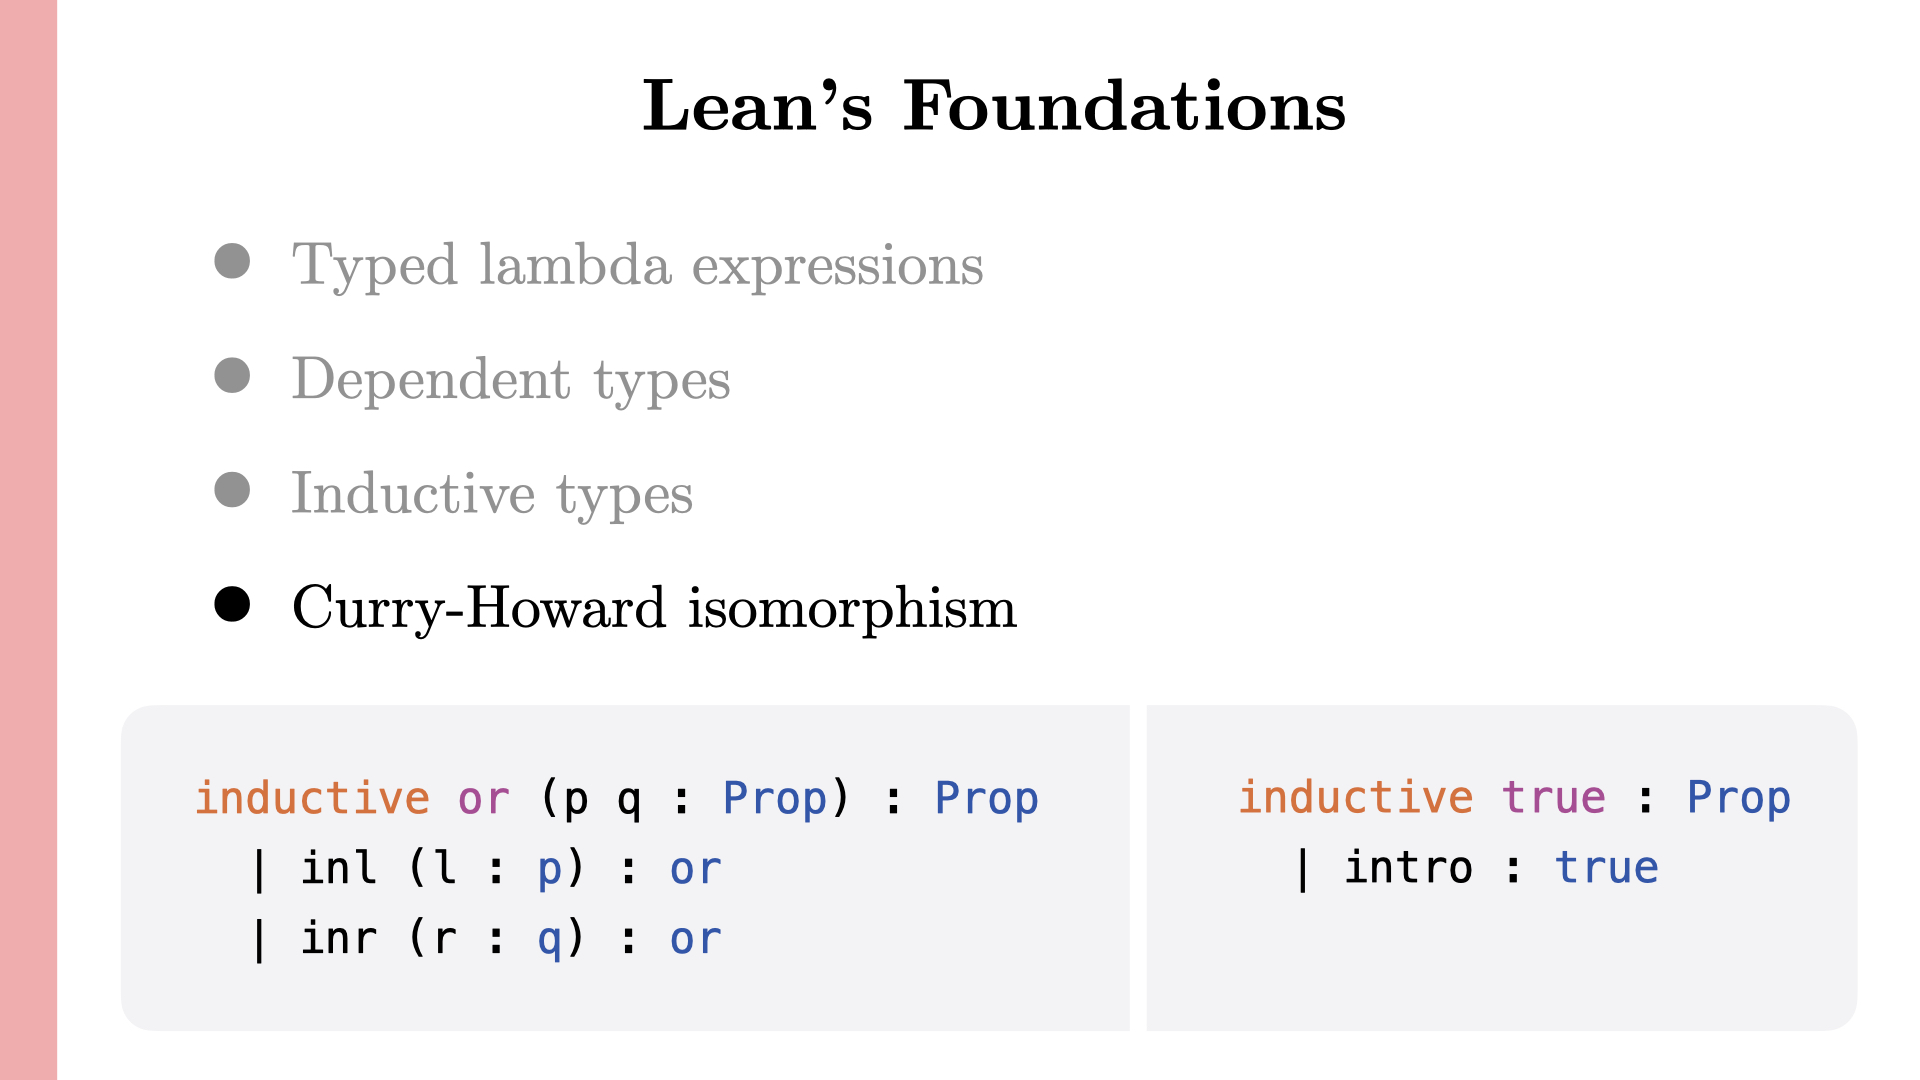
\includegraphics[width=\columnwidth]{Slides/Slide 7.jpeg}
\end{center}

In the context of Lean, the Curry-Howard isomorphism is the answer the
question: How do we express proofs in type theory? There's really not a
\emph{correct} answer to this question, but one neat approach was
discovered by Haskell Curry: We model propositions as types and proofs
as instances of those types. There might be some questions that might
come with this, which are hopefully clarified by the examples at the
bottom. Firstly, how do we express proposition as types - aren't they
terms over values? In short, with types that are dependent over values.
For example, consider how we formalize a disjunction with the
\lstinline{or} type: If \lstinline{p} and \lstinline{q} are already propositions,
then the proposition \emph{p ∨ q} is the type \lstinline{or p q}. The way
we declare \lstinline{p} and \lstinline{q} to be propositions, is by declaring
their type to be \lstinline{Prop}. Recall that we model propositions as
types. So \lstinline{p} and \lstinline{q} are types, and hence, \lstinline{Prop}
is again a type of types, similar to \lstinline{Type*}. By the Curry-Howard
isomorphism we also defined proofs to be instances of the propositions
we want to prove. So the definition of \lstinline{or} also shows us how we
can create proofs of a disjunction: Either by providing a proof of
\lstinline{p} using the \lstinline{inl} constructor, or by providing a proof
of \lstinline{q} using the \lstinline{inr} constructor. That is, \lstinline{l}
and \lstinline{r} are proofs of \lstinline{p} and \lstinline{q} respectively. As
another example of a proposition, consider \lstinline{true}? What this
definition tells us, is that we can simply construct an instance of
\lstinline{true} using the \lstinline{intro} constructor. We don't require
proofs of any other propositions for this. Hence, we can always obtain a
proof of the proposition \lstinline{true} out of thin air. Of course,
that's exactly how \lstinline{true} should behave. We can define all
fundamental propositional connectives in Lean using this approach. And
in fact, one of the observations of the Curry-Howard isomorphism was the
correspondence of these logical connectives to ``normal, data-related
types''.

\begin{center}
  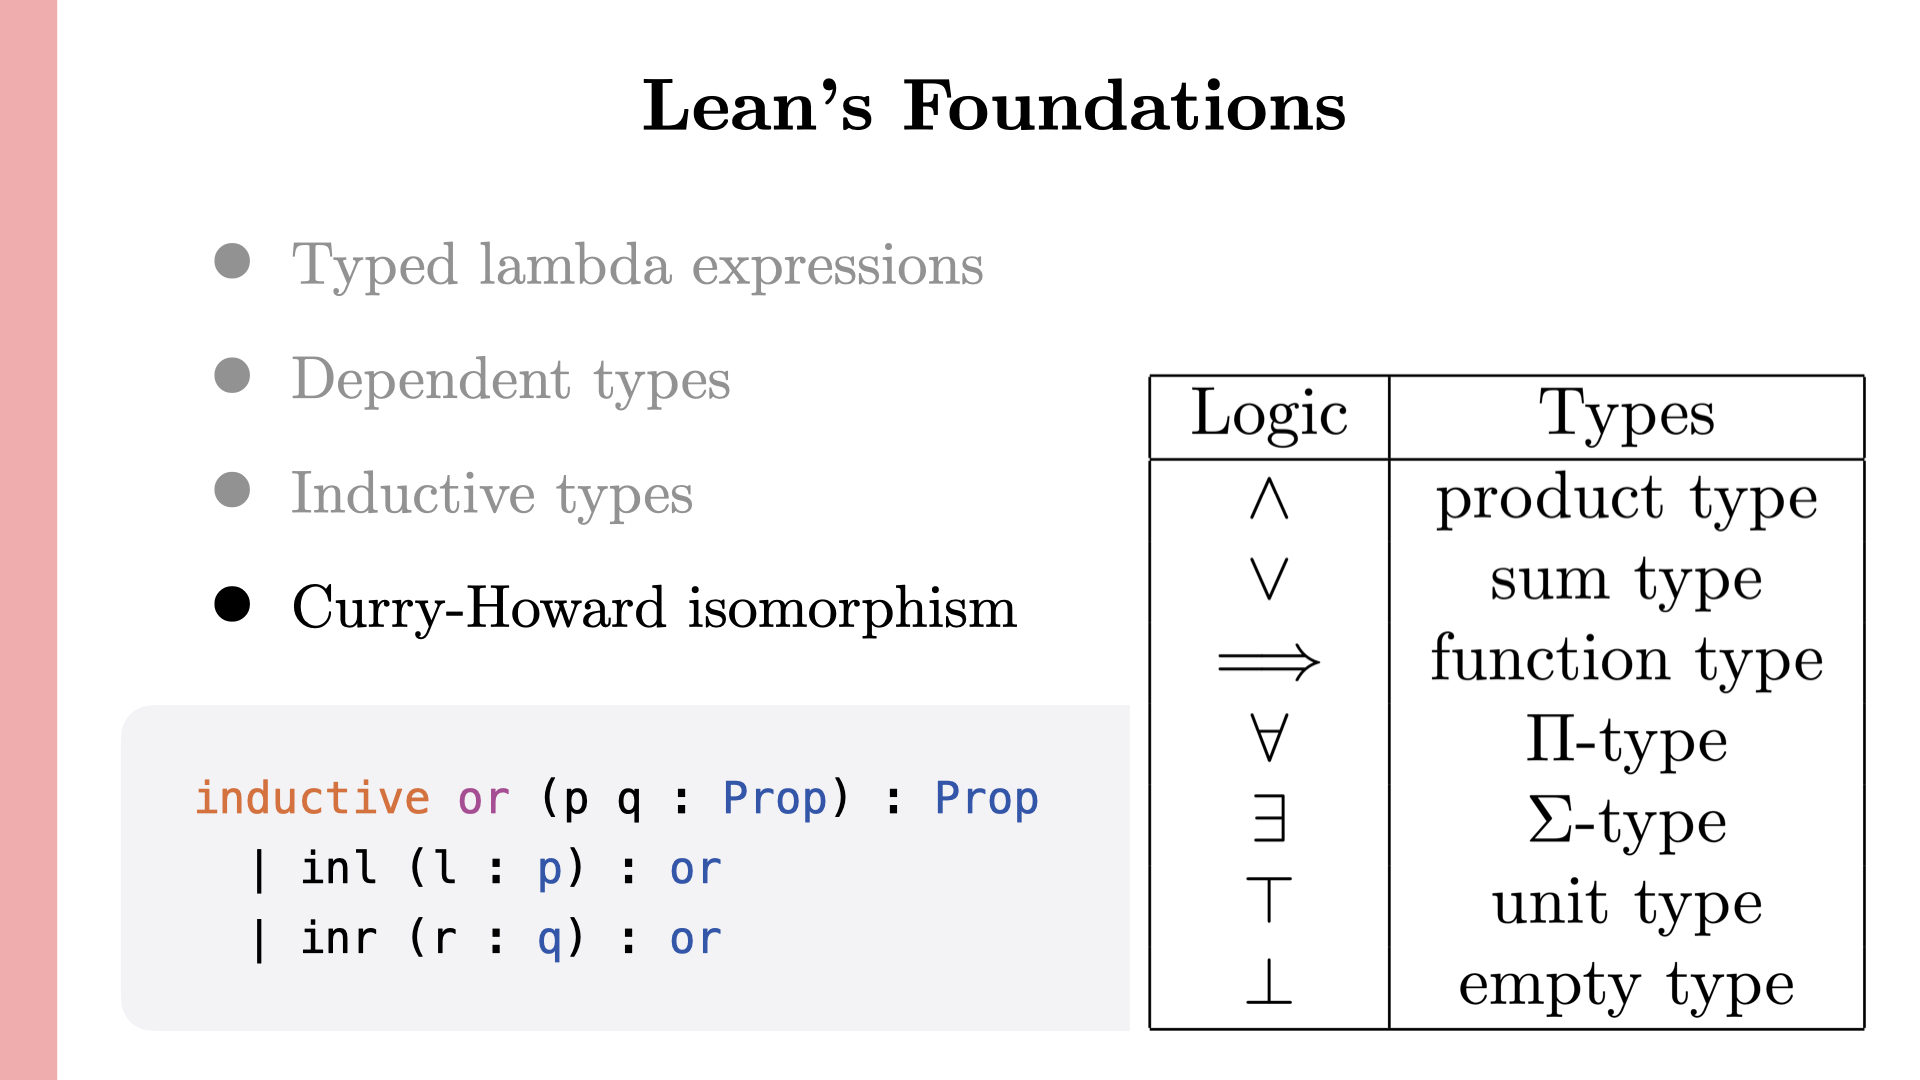
\includegraphics[width=\columnwidth]{Slides/Slide 8.jpeg}
\end{center}

For example, the \lstinline{or} type corresponds to what is known as a
\emph{sum type}, i.e. a type that can hold a value of one type or
another (this is also called a \emph{discriminated union} in traditional
programming languages). The \lstinline{true} type corresponds to a unit
type, that is a type that has only one possible value (this corresponds
to the \lstinline{void} type in C). One of my favorite correspondences is
between implication and function types. That is, a proof of an
implication \emph{A ⇒ B} corresponds to a function that can map a proof
of \emph{A} to a proof of \emph{B}. Hence, in Lean the implication arrow
is in fact exactly the same construct as the function arrow. While the
\emph{propositions as types} paradigm \emph{technically} provides us
with a way to construct proofs, it's really not a fun way of proving
things. As humans, we tend to write proofs as sequences of expressions
that lead us toward a proof goal bit by bit. This approach isn't really
possible when directly constructing proofs as instances of types.

To solve this problem, Lean provides us with a way of proving
propositions using a sequential approach, called \emph{tactic mode}. To
demonstrate tactics, I would like to prove something about reactors with
you, which is actually part of the formalization of the Reactor model in
my thesis. We're going to formalize and prove an (admittedly trivial)
theorem about ports.

\begin{center}
  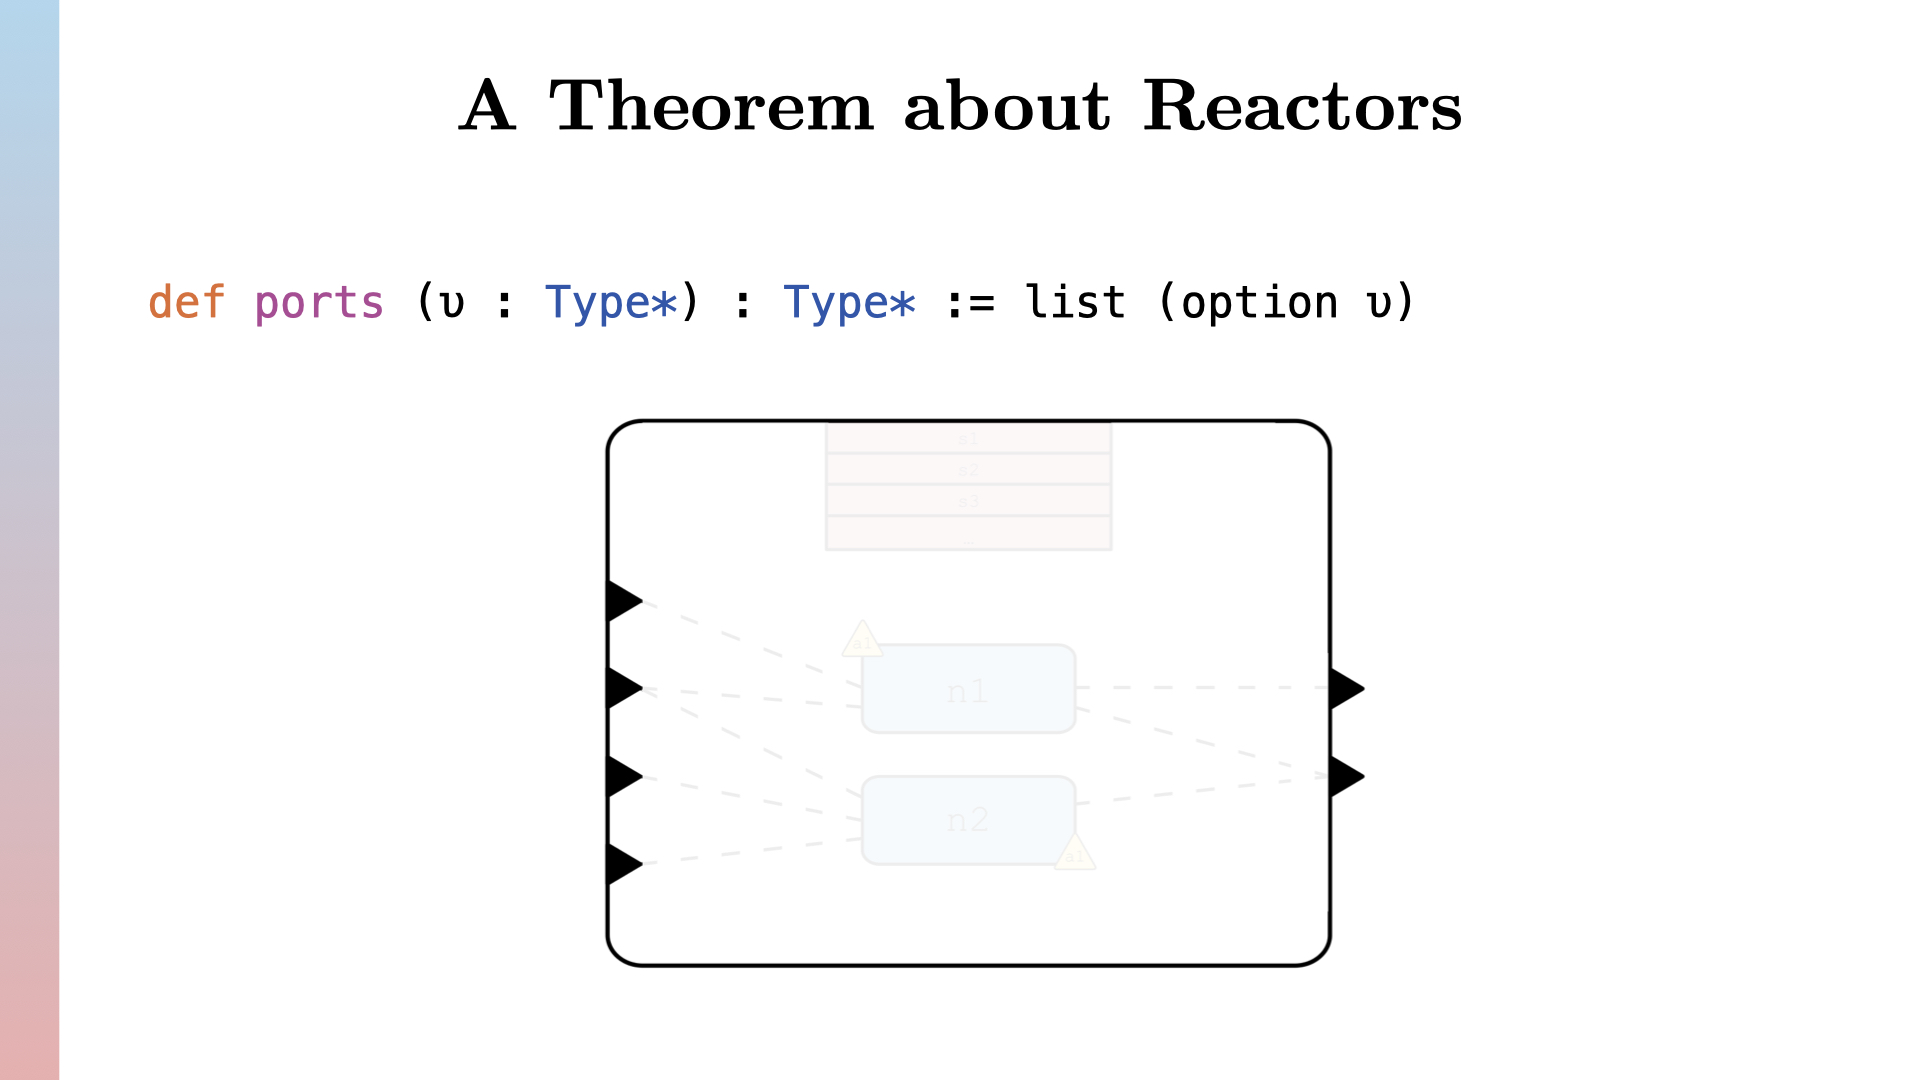
\includegraphics[width=\columnwidth]{Slides/Slide 9.jpeg}
\end{center}

We define ports as lists over optional values. That is, first of all
\lstinline{ports} is a \emph{type}, indicated by the type annotation
\lstinline{: Type*}. On the right-hand side, we declare what exact type
\lstinline{ports} is: a list over instances of \lstinline{option υ}. The
\lstinline{υ} is the type of \emph{values}. Recall that the Reactor model
defines values as \emph{opaque} objects, which are passed around between
reactors and reactions. Hence, we model them like a generic type by
defining them using a dependent parameter. Lastly, the \lstinline{option}
is just responsible for equipping the values with an \emph{absent value}
(as defined in the Reactor model). This isn't really important to us
now. Thus, \lstinline{ports} is a type that models lists of values. We can
refer to each individual port by indexing into these lists. In the
process of formalizing the Reactor model, at some point I needed to be
able to check whether two instances of \lstinline{ports} have the same
values for given indices --- for example, whether the second and the fifth
port of two instances hold the same value. To express what it would mean
for two instances of \lstinline{ports} to have this correspondence, we can
define a proposition: \lstinline{eq_at}.

\begin{center}
  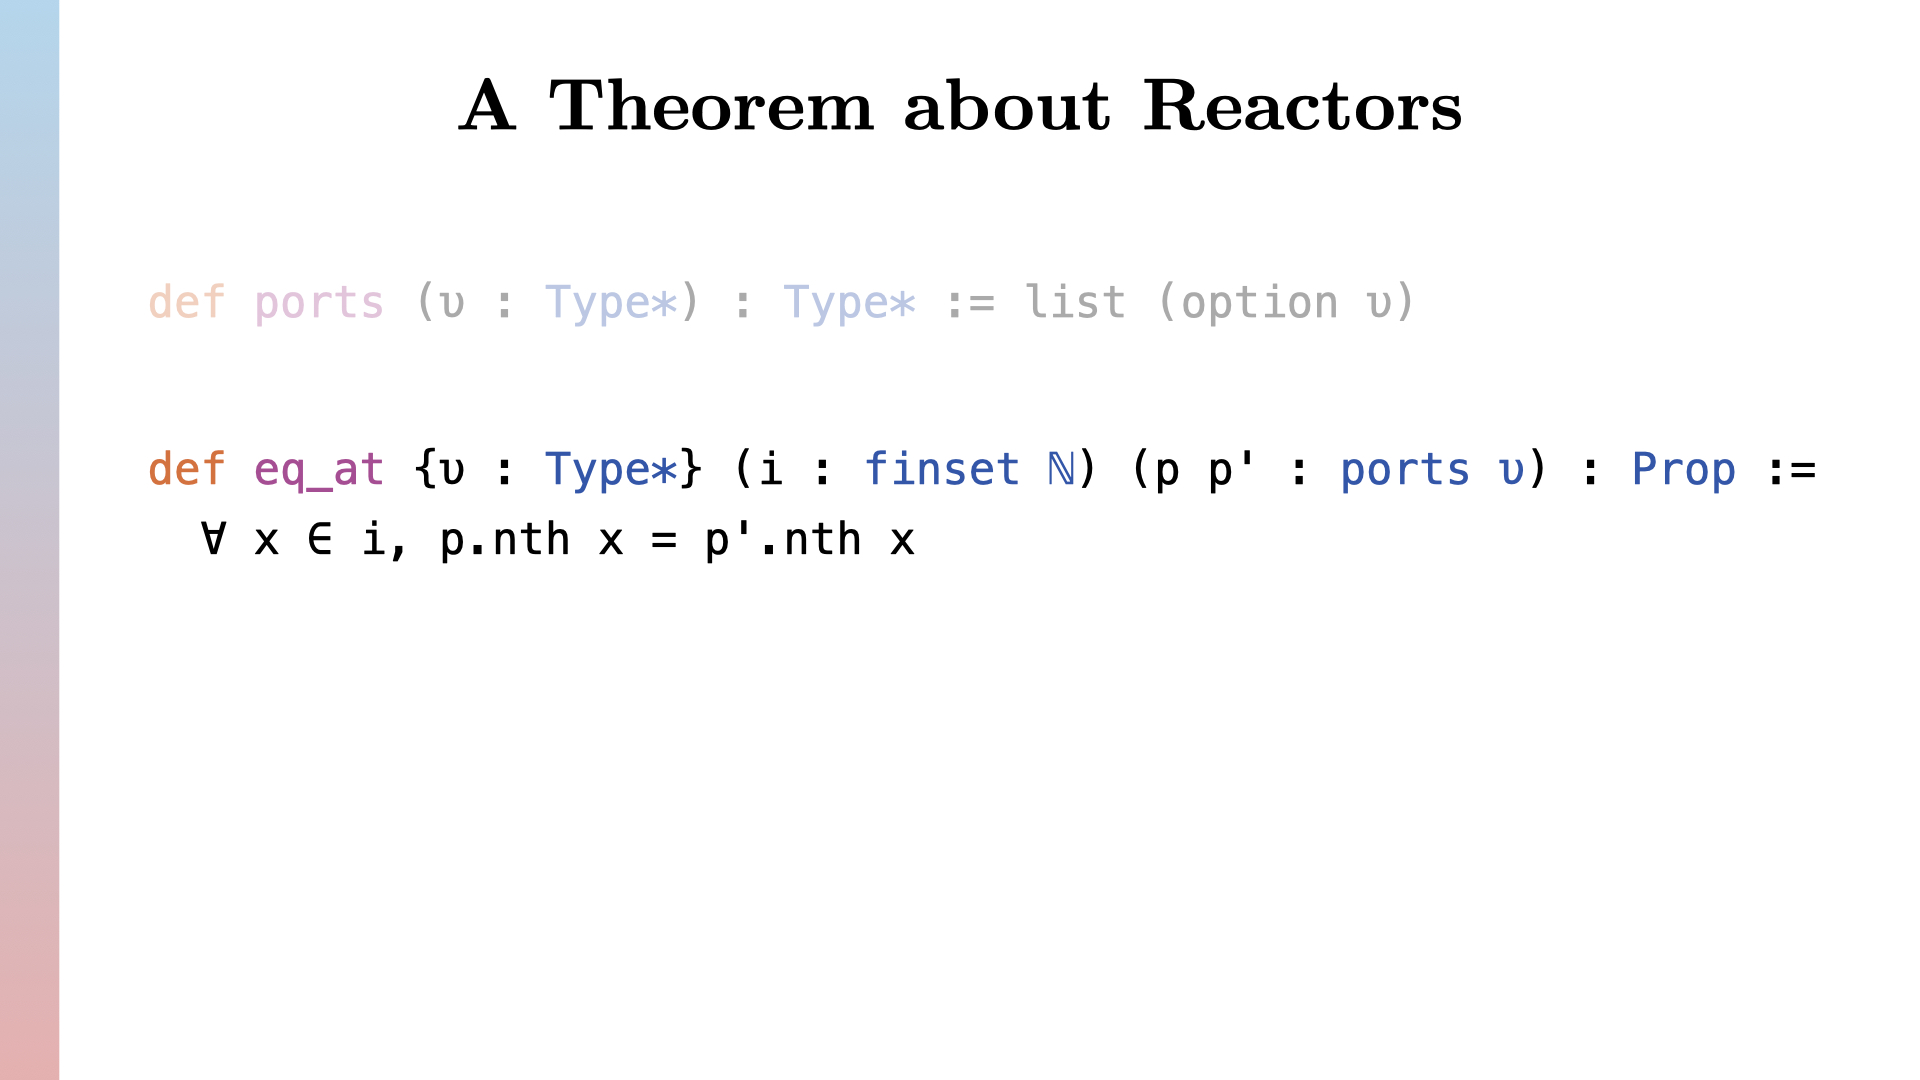
\includegraphics[width=\columnwidth]{Slides/Slide 10.jpeg}
\end{center}

That is, \lstinline{eq_at} \emph{is} a proposition (indicated by the
\lstinline{: Prop}). Namely, the proposition that for each index
\lstinline{x} from the set of indices \lstinline{i}, the instances \lstinline{p}
and \lstinline{p'} have corresponding values at \lstinline{x}
(the function \lstinline{nth} gets the value at the given index).

What I would like to prove now (with your help) is that \lstinline{eq_at}
is reflexive.

\begin{center}
  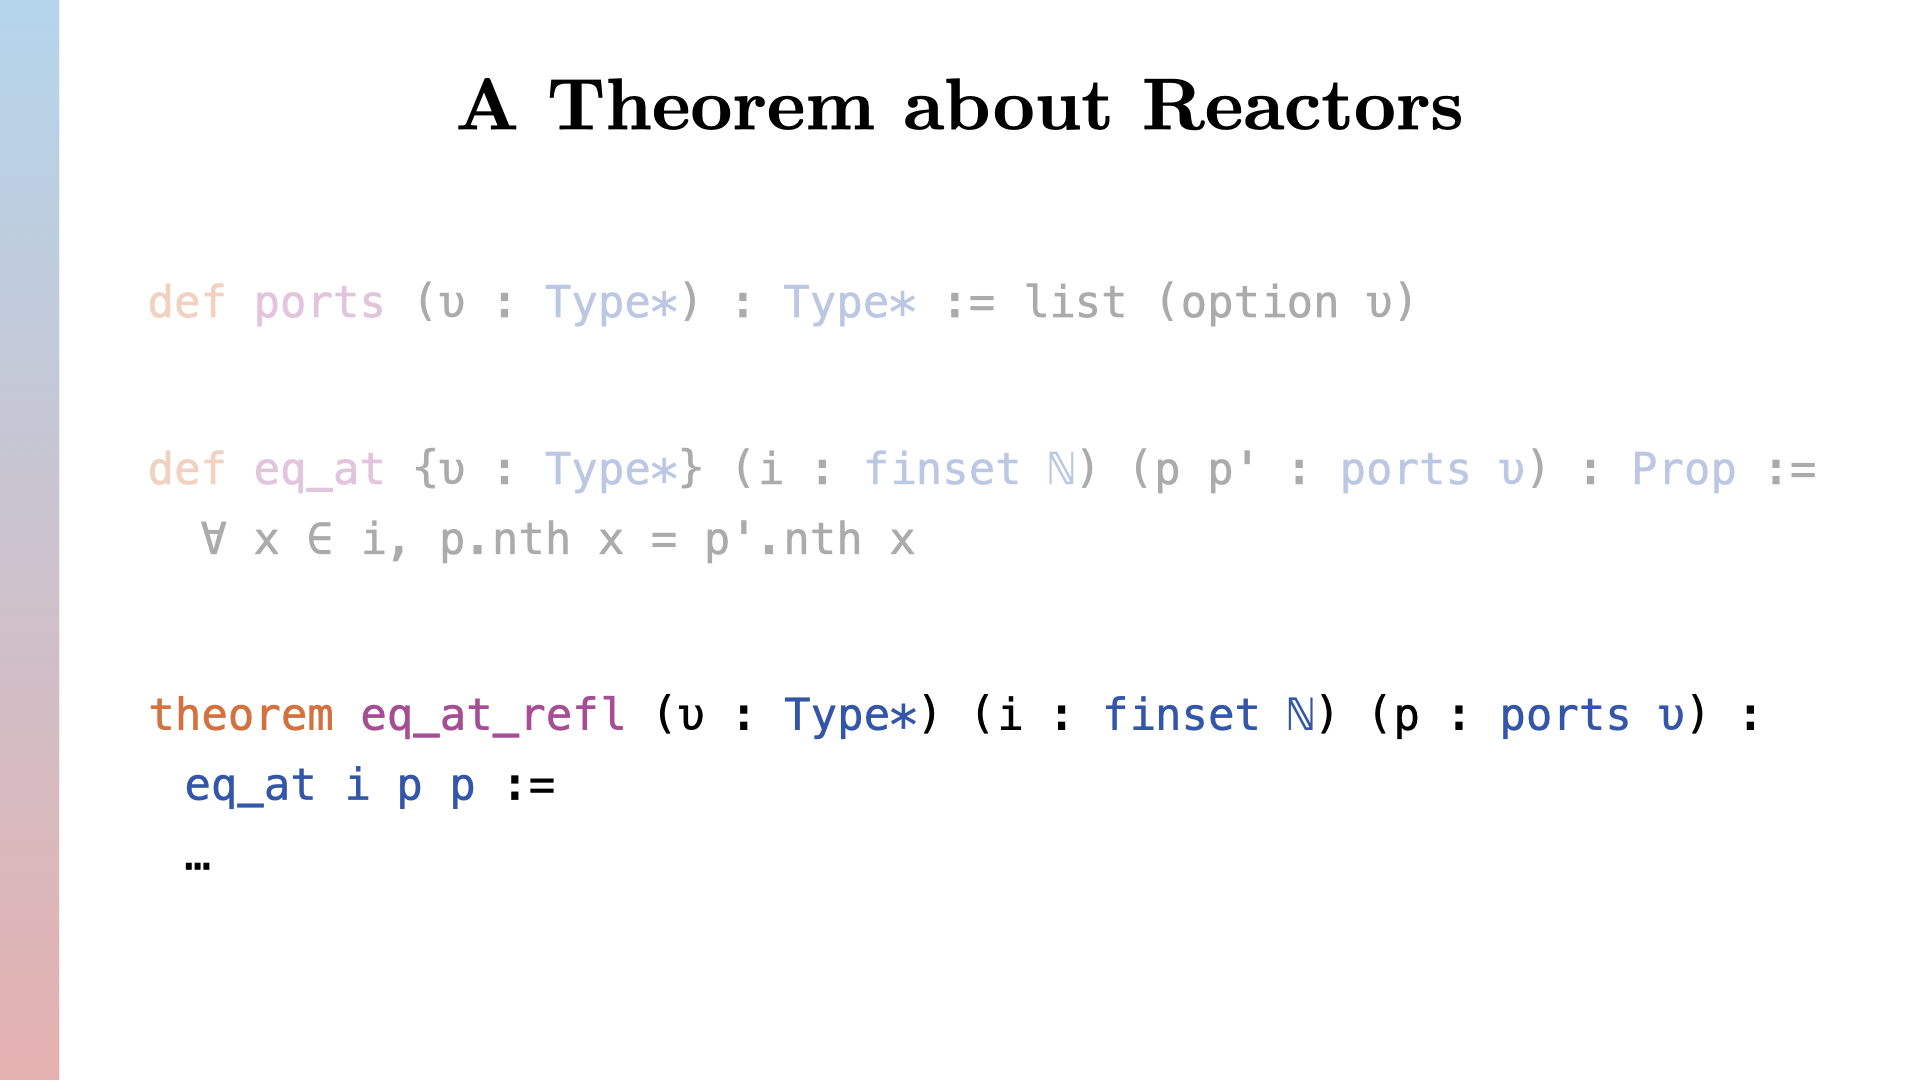
\includegraphics[width=\columnwidth]{Slides/Slide 11.jpeg}
\end{center}

That is, given any set of indices \lstinline{i} and any instance of
\lstinline{ports} \lstinline{p}, it will always hold that
\lstinline{eq_at i p p}. I hope you see why this is trivially true.
What isn't trivial, is how to prove this theorem. First of all, let's
consider its definition. We declare theorems in Lean using the
\lstinline{theorem} keyword. The type of a theorem is a proposition: the
one we intend to prove. This works, because (if you recall) propositions
are types and hence \lstinline{eq_at i p p} (since it is a proposition)
is a type. Since a proof of a proposition is just an instance of it,
proving a theorem means construction an instance of its type. In this
case, an instance of type \lstinline{eq_at i p p} looks like this.

\begin{center}
  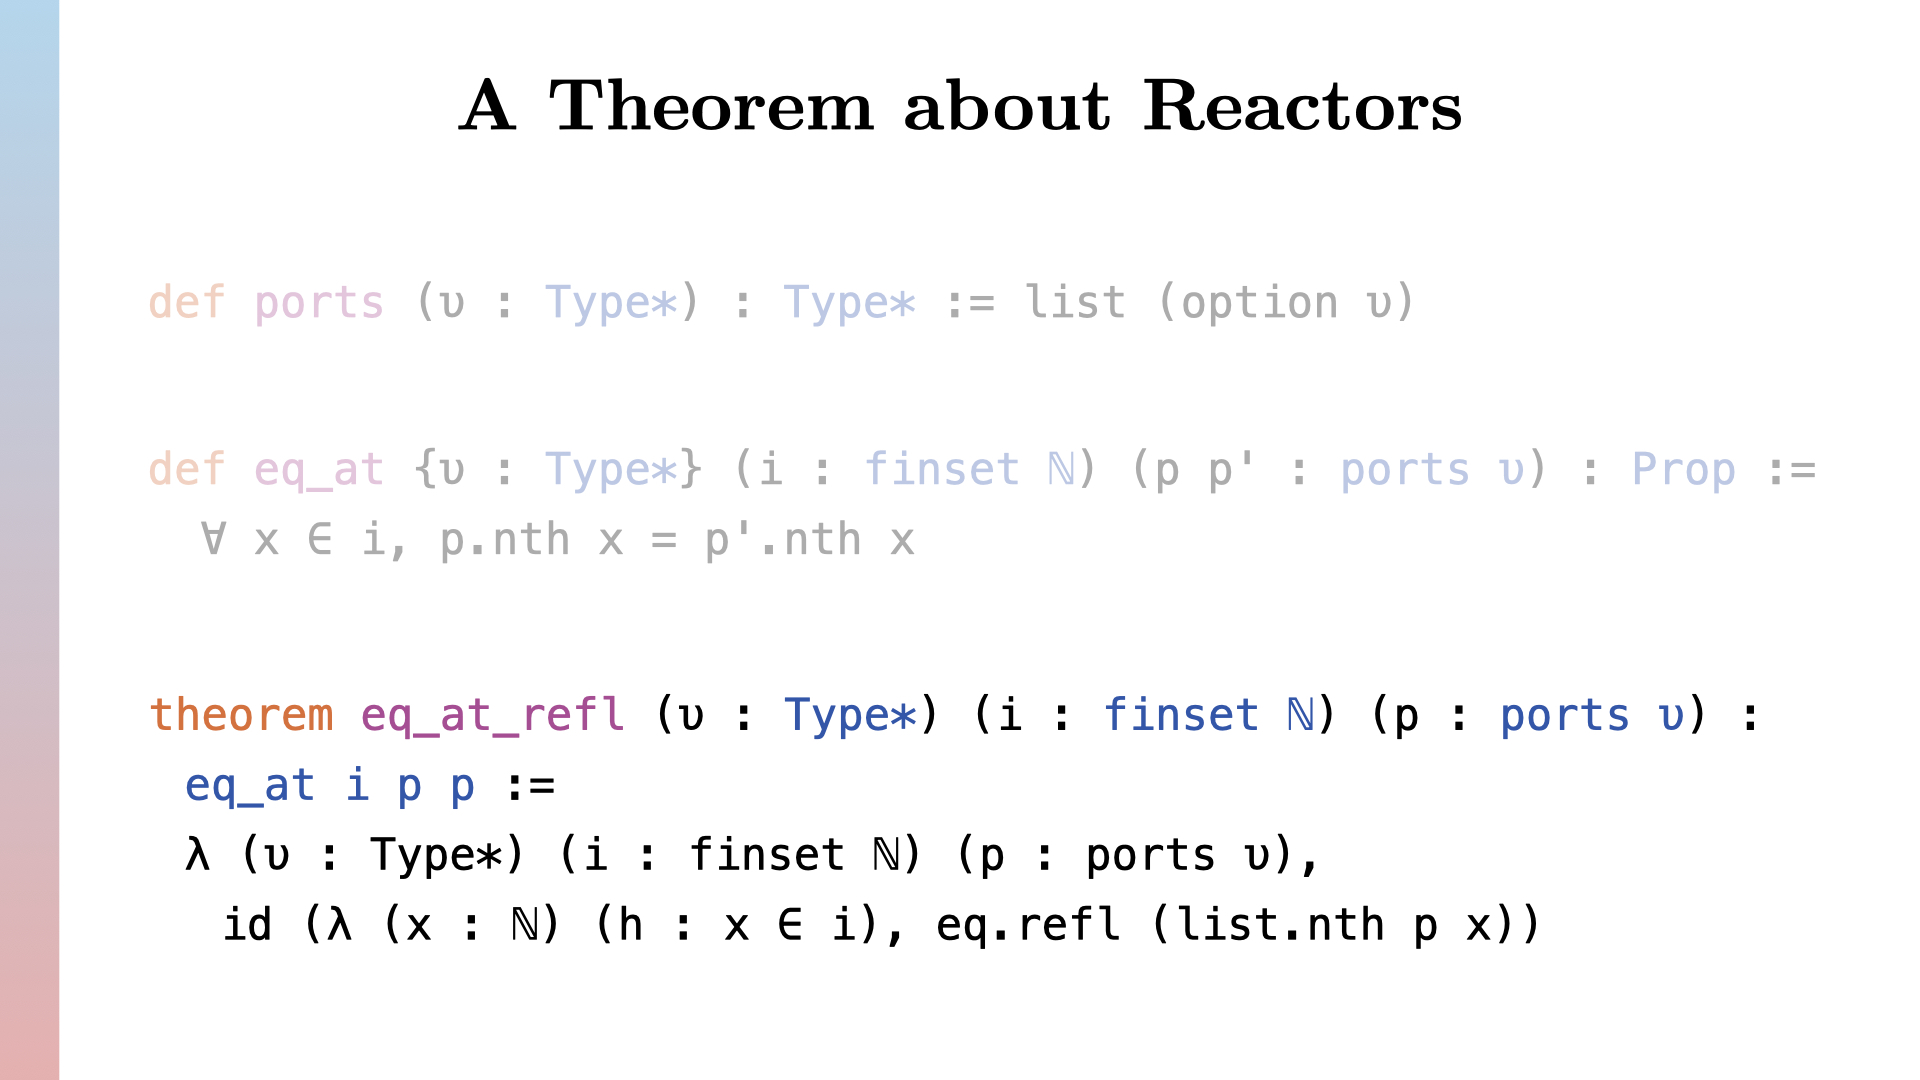
\includegraphics[width=\columnwidth]{Slides/Slide 12.jpeg}
\end{center}

This is, of course, of no help to our human brains. So let's try proving
this theorem using tactic mode instead.

\begin{center}
  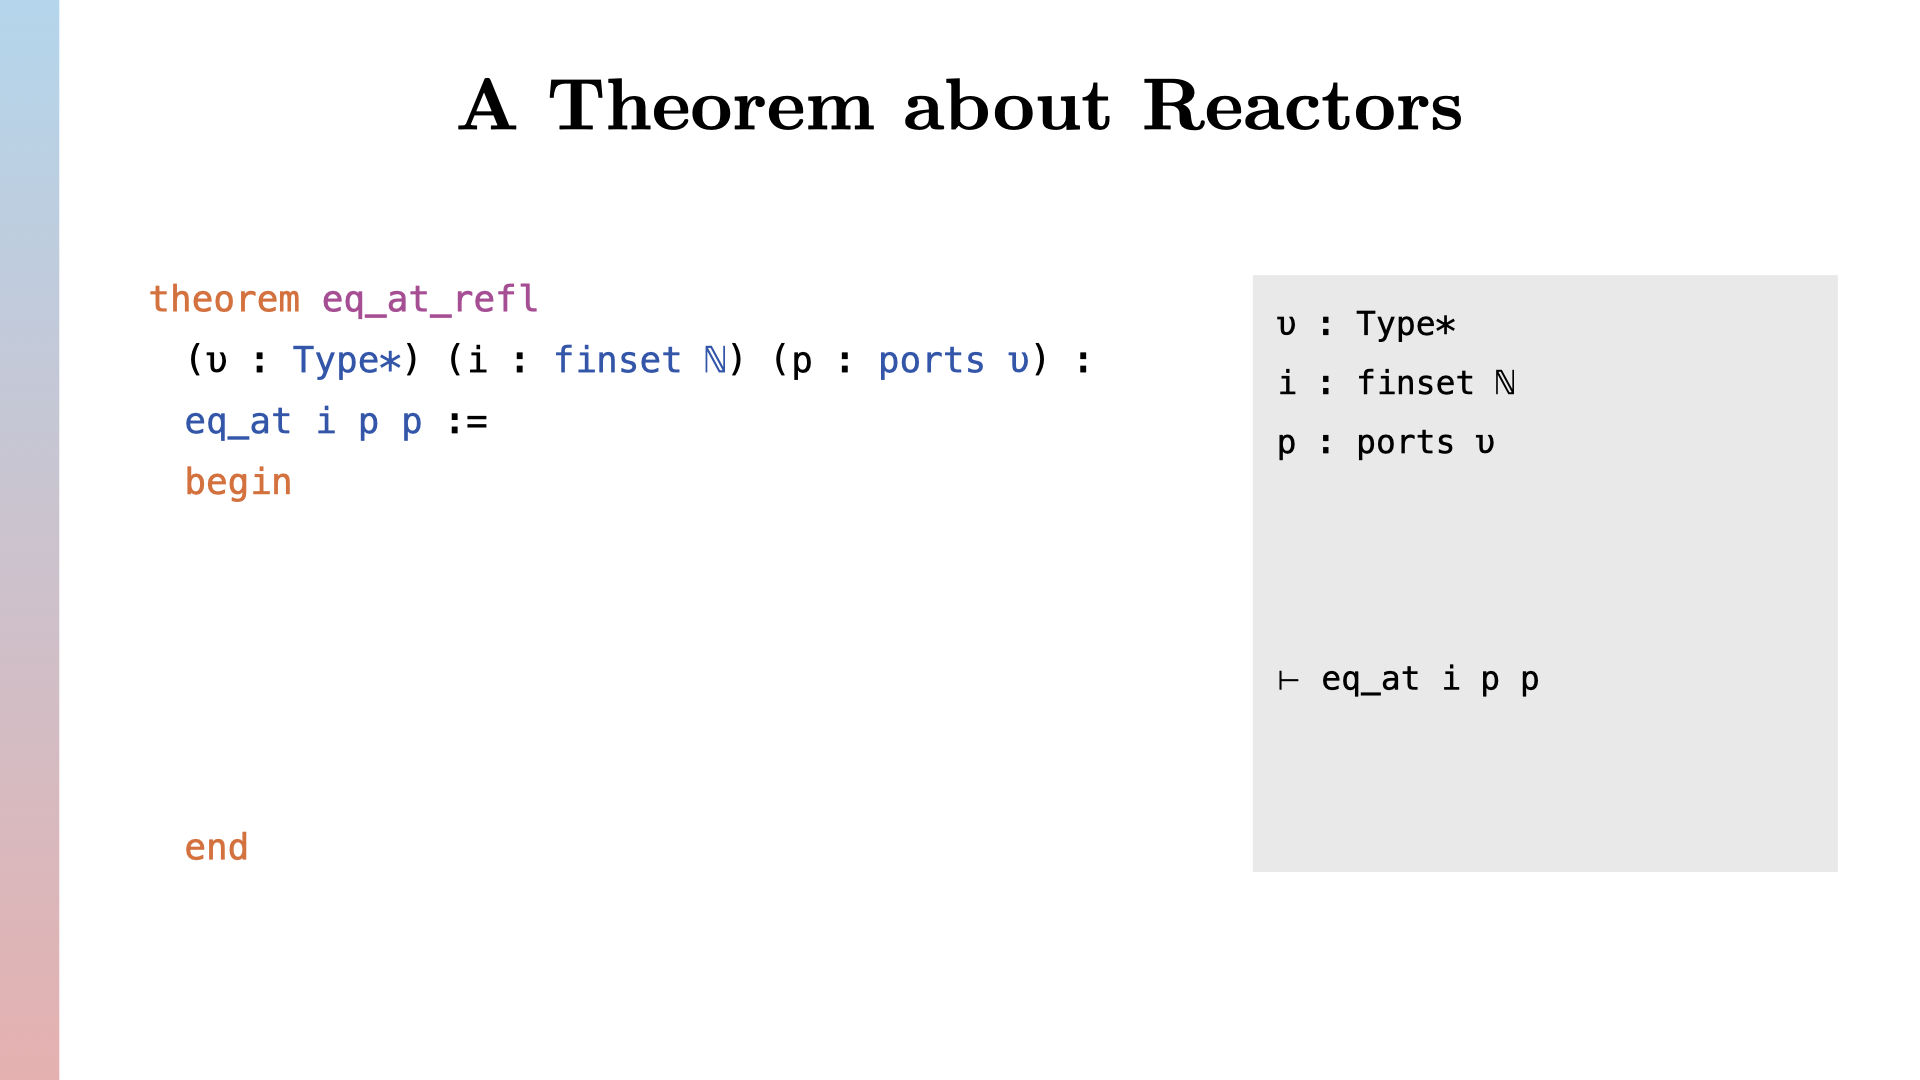
\includegraphics[width=\columnwidth]{Slides/Slide 13.jpeg}
\end{center}

We enter tactic mode using these \lstinline{begin} and \lstinline{end}
delimiters. Once we're in tactic mode, we can see why Lean is also
called a \emph{proof assistant}: It's going to help us keep track of our
proof by visualizing what is called the \emph{goal state} on the right.
Here we get information about the hypotheses/assumptions we've made so
far, as well as the remaining goal (after the \lstinline{⊢}) we need to
prove in order to complete the proof of the theorem. In the beginning,
our goal is precisely the proposition of the theorem. Our aim is now to
simplify this goal, to the point where we can prove it by using other
theorems or axioms. So the first step we'll take here, is to unfold the
definition of \lstinline{eq_at}.

\begin{center}
  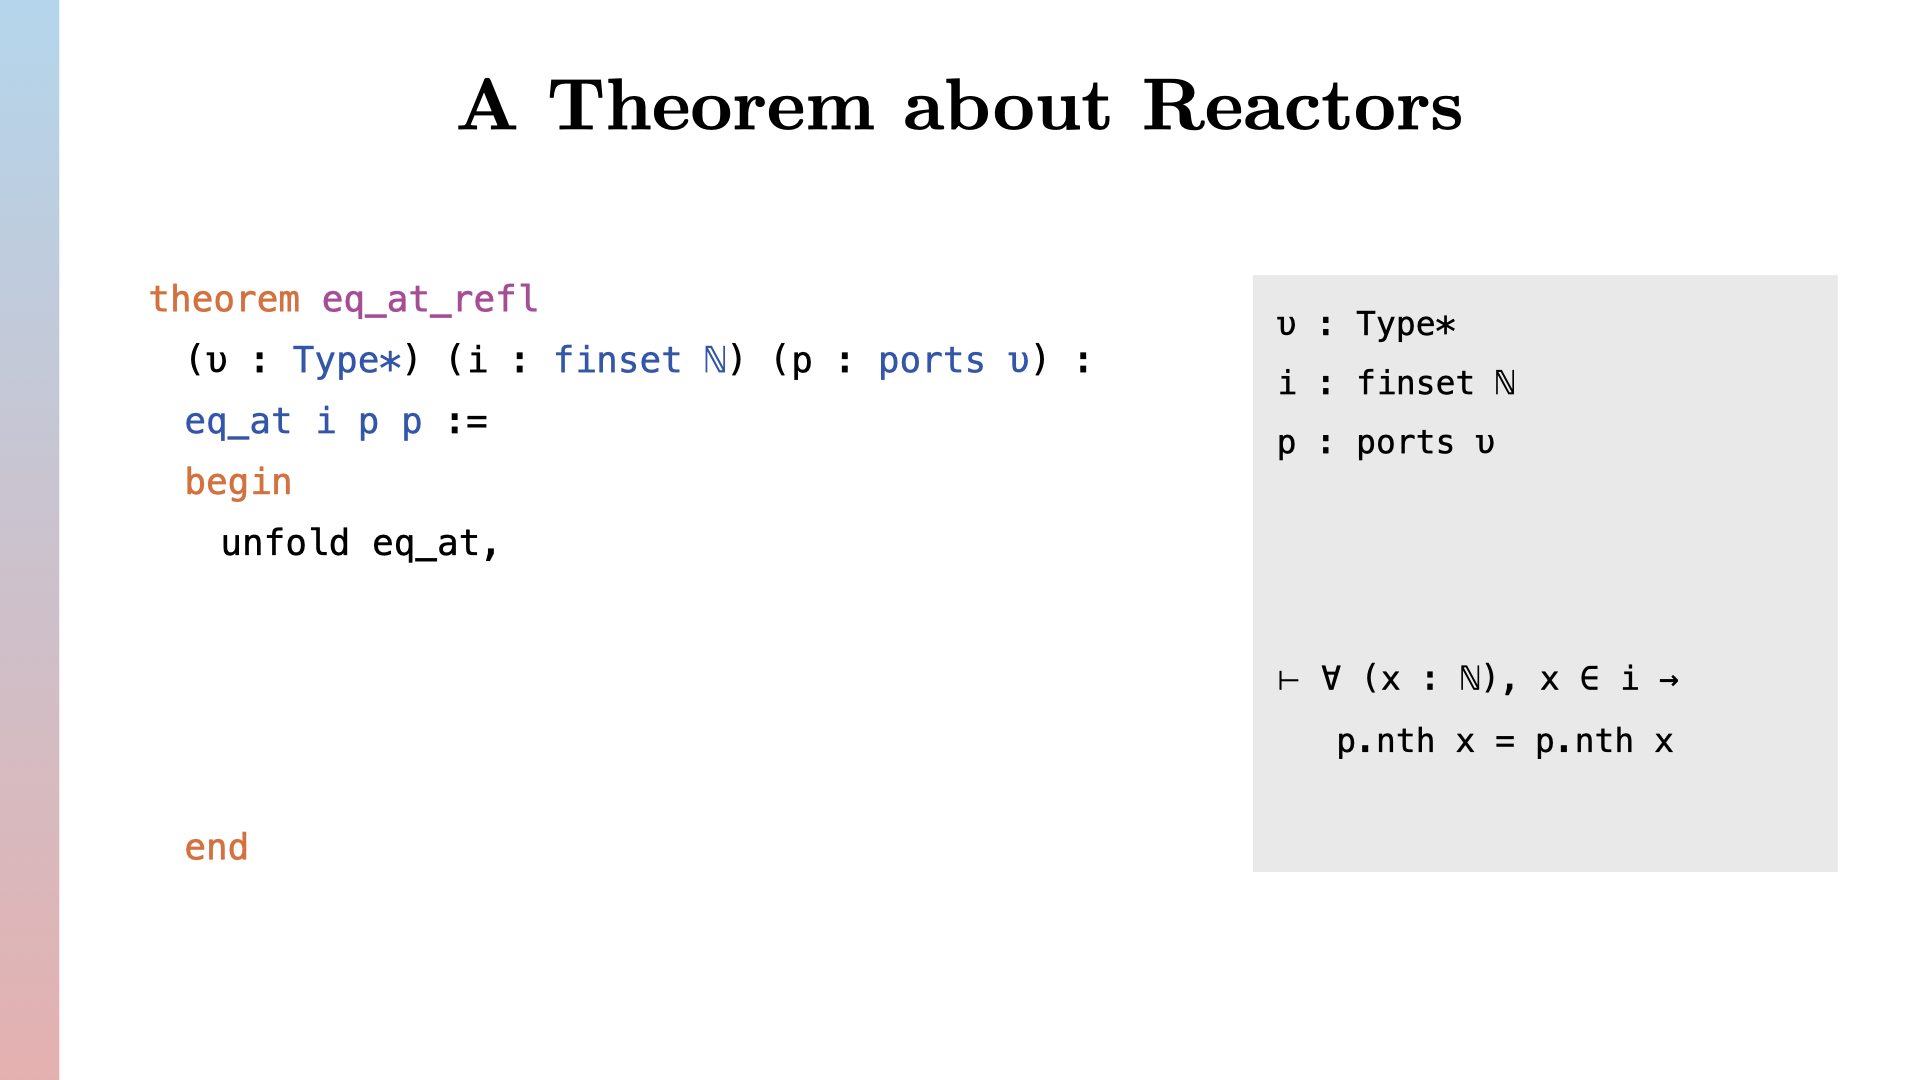
\includegraphics[width=\columnwidth]{Slides/Slide 14.jpeg}
\end{center}

Unfolding the definition changed our goal. Hence, we now need to prove a
specific ∀-proposition. Now, this is where I would like your feedback as
intelligent human proof assistants: If you're trying to prove a
proposition \emph{for all elements} of some set (or \emph{type} in this
case), how do you go about that? Exactly, you introduce an arbitrary but
fixed element from that set and show that the theorem holds for that
arbitrary element. We can do exactly this with the \lstinline{intro}
tactic.

\begin{center}
  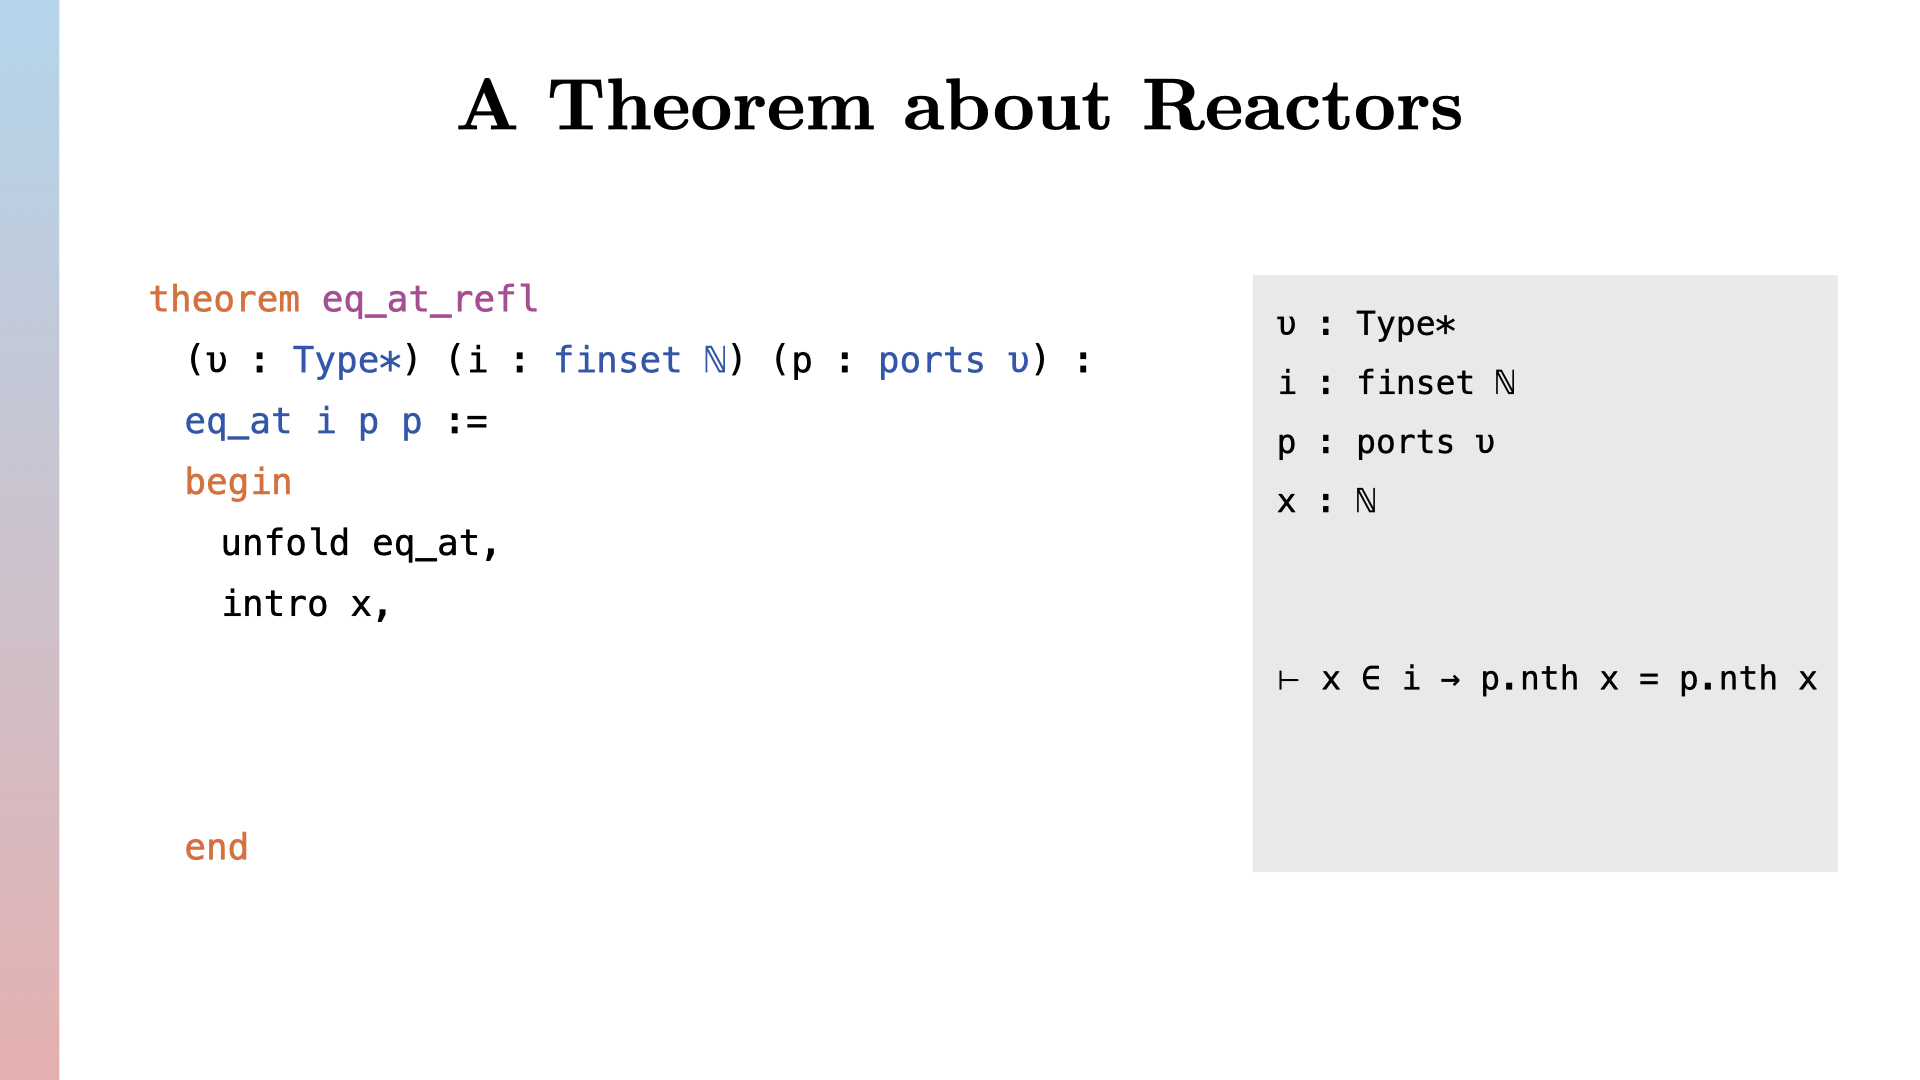
\includegraphics[width=\columnwidth]{Slides/Slide 15.jpeg}
\end{center}

As you can see, not only does this change our goal state, but we've also
introduced a new assumption. So now we need to prove an implication.
Again I would like to get some feedback from you: If you're trying to
prove an implication, how do you go about that? Exactly, you assume the
premise to be true and then show that the consequence must hold. For
this, we can again use the \lstinline{intro} tactic.

\begin{center}
  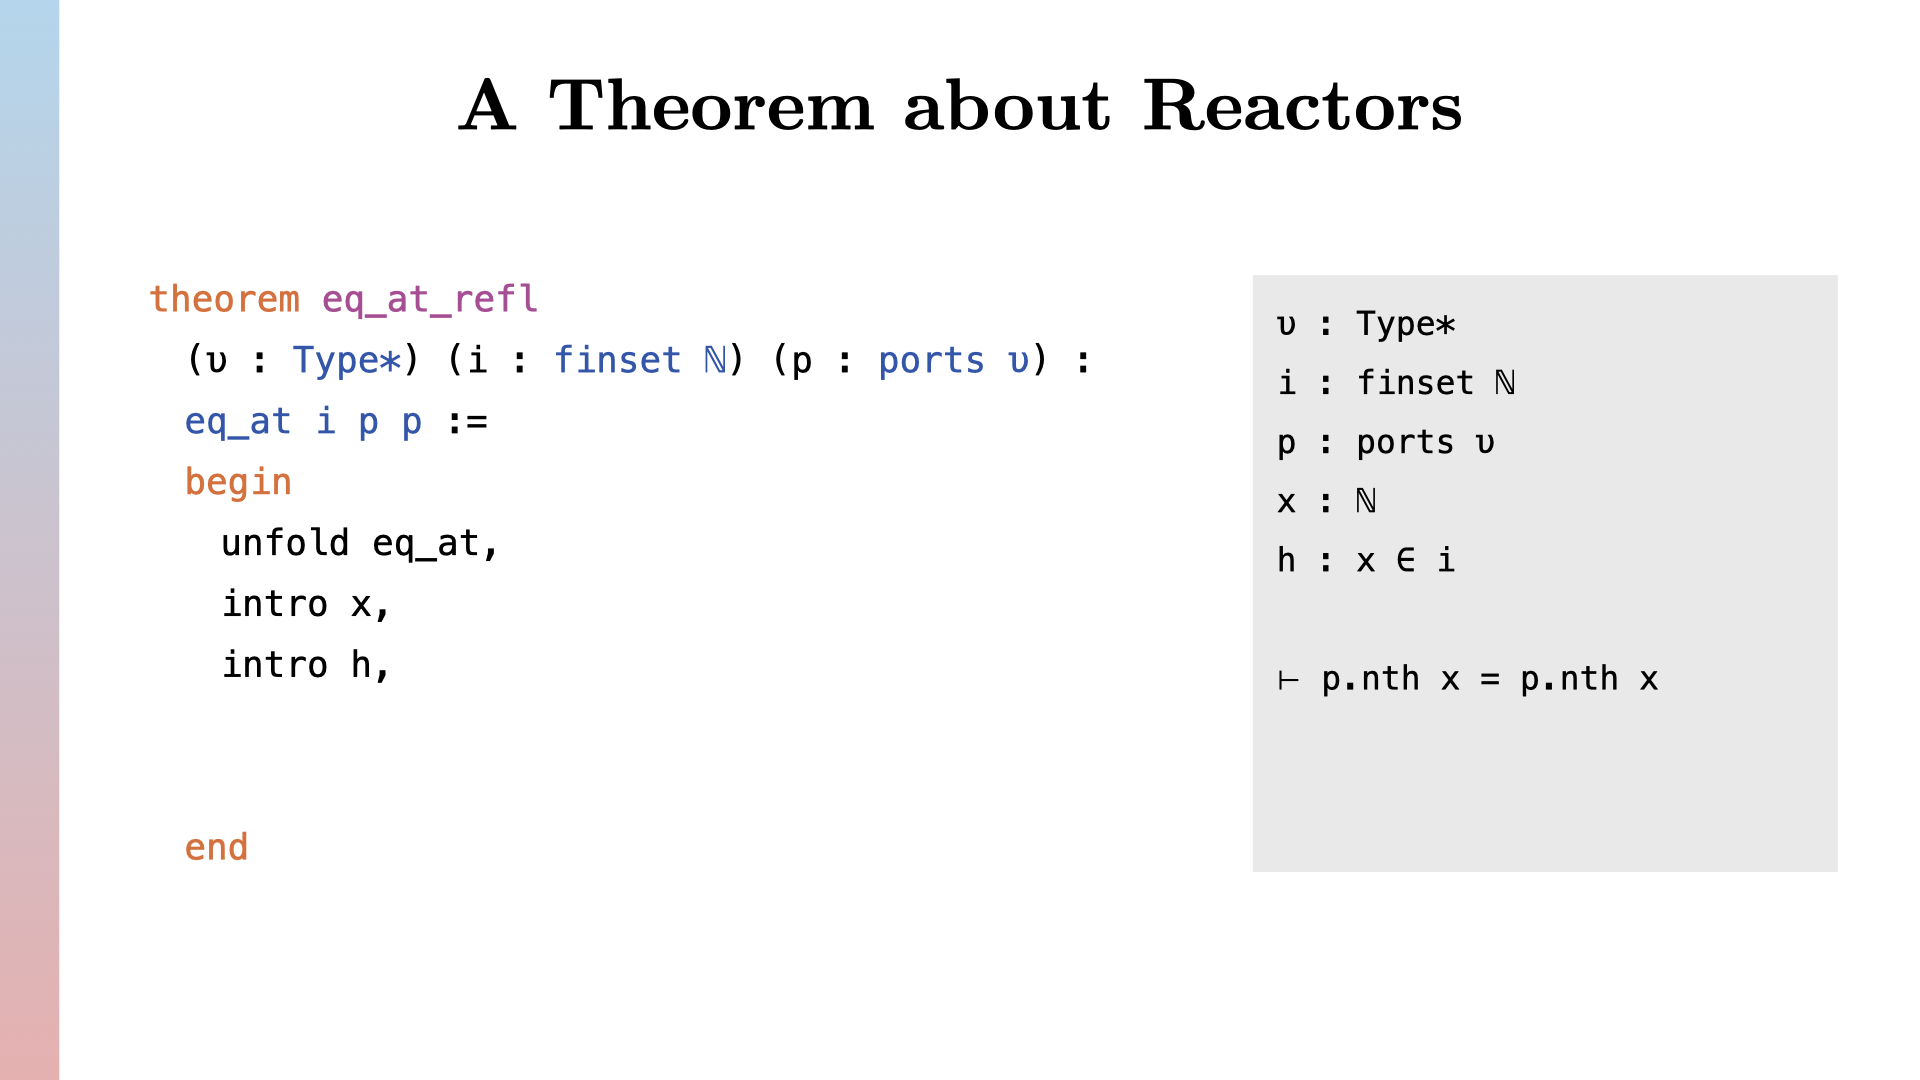
\includegraphics[width=\columnwidth]{Slides/Slide 16.jpeg}
\end{center}

Now all that's left to show is that \lstinline{p.nth x} is equal to
itself. There's a really simple way to do this, but I'll take the longer
route here, just to demonstrate some more tactics. First of all, there's
a really nice theorem in Lean called \lstinline{congr_arg}, which states
that if a function is called with equal arguments, then the result must
be the same. We can apply this theorem to out goal using the
\lstinline{apply} tactic.

\begin{center}
  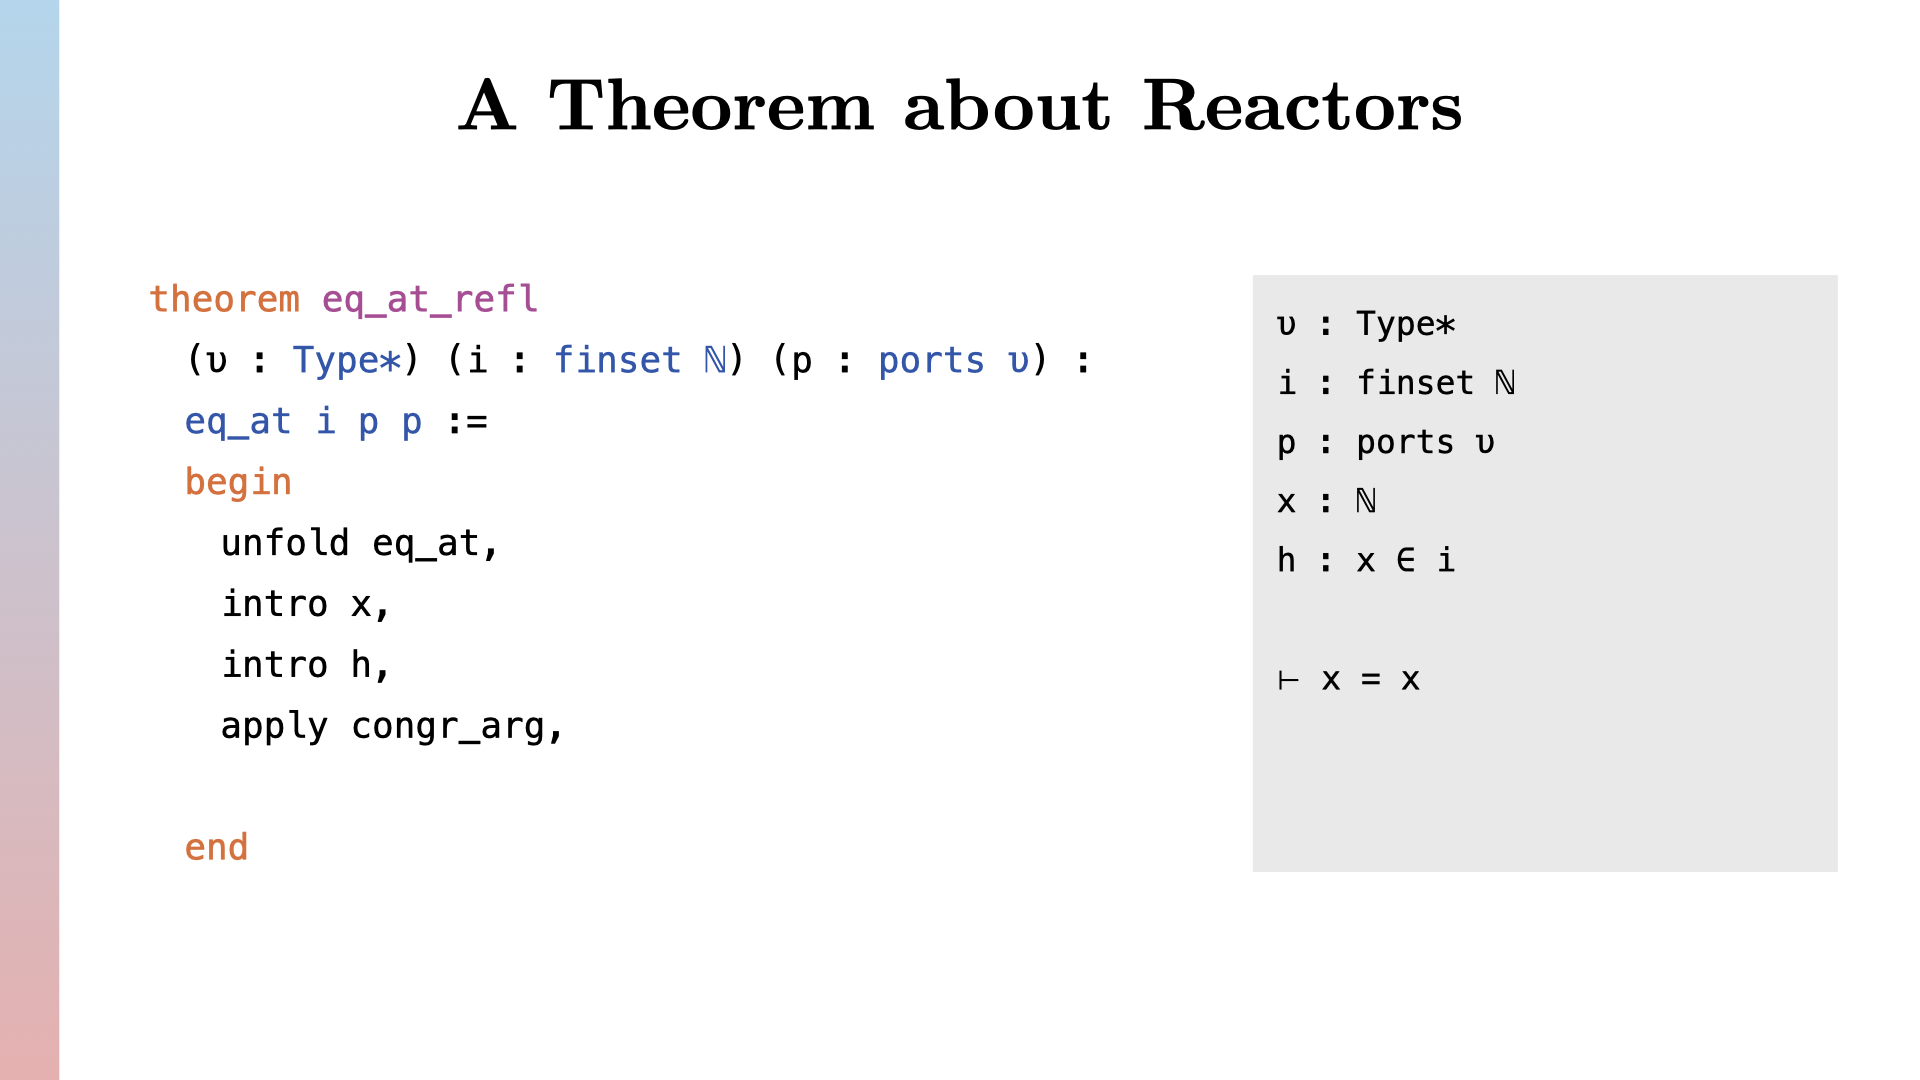
\includegraphics[width=\columnwidth]{Slides/Slide 17.jpeg}
\end{center}

This is the point where you get to experience Lean in its full glory,
because we aren't done yet. We now need to prove that the arguments to
the function are in fact equal, i.e.~that \lstinline{x = x}. How do you
prove that a thing is equal to itself? --- by the definition of equality.
In Lean, the equality-proposition is a defined just like the \lstinline{or}
and \lstinline{true} propositions: as an inductive type. It has a
constructor that we can call, where we pass in some object and in return
get a proof that that object is equal to itself. We can tell Lean that
this instance is precisely our remaining goal by using the
\lstinline{exact} tactic.

\begin{center}
  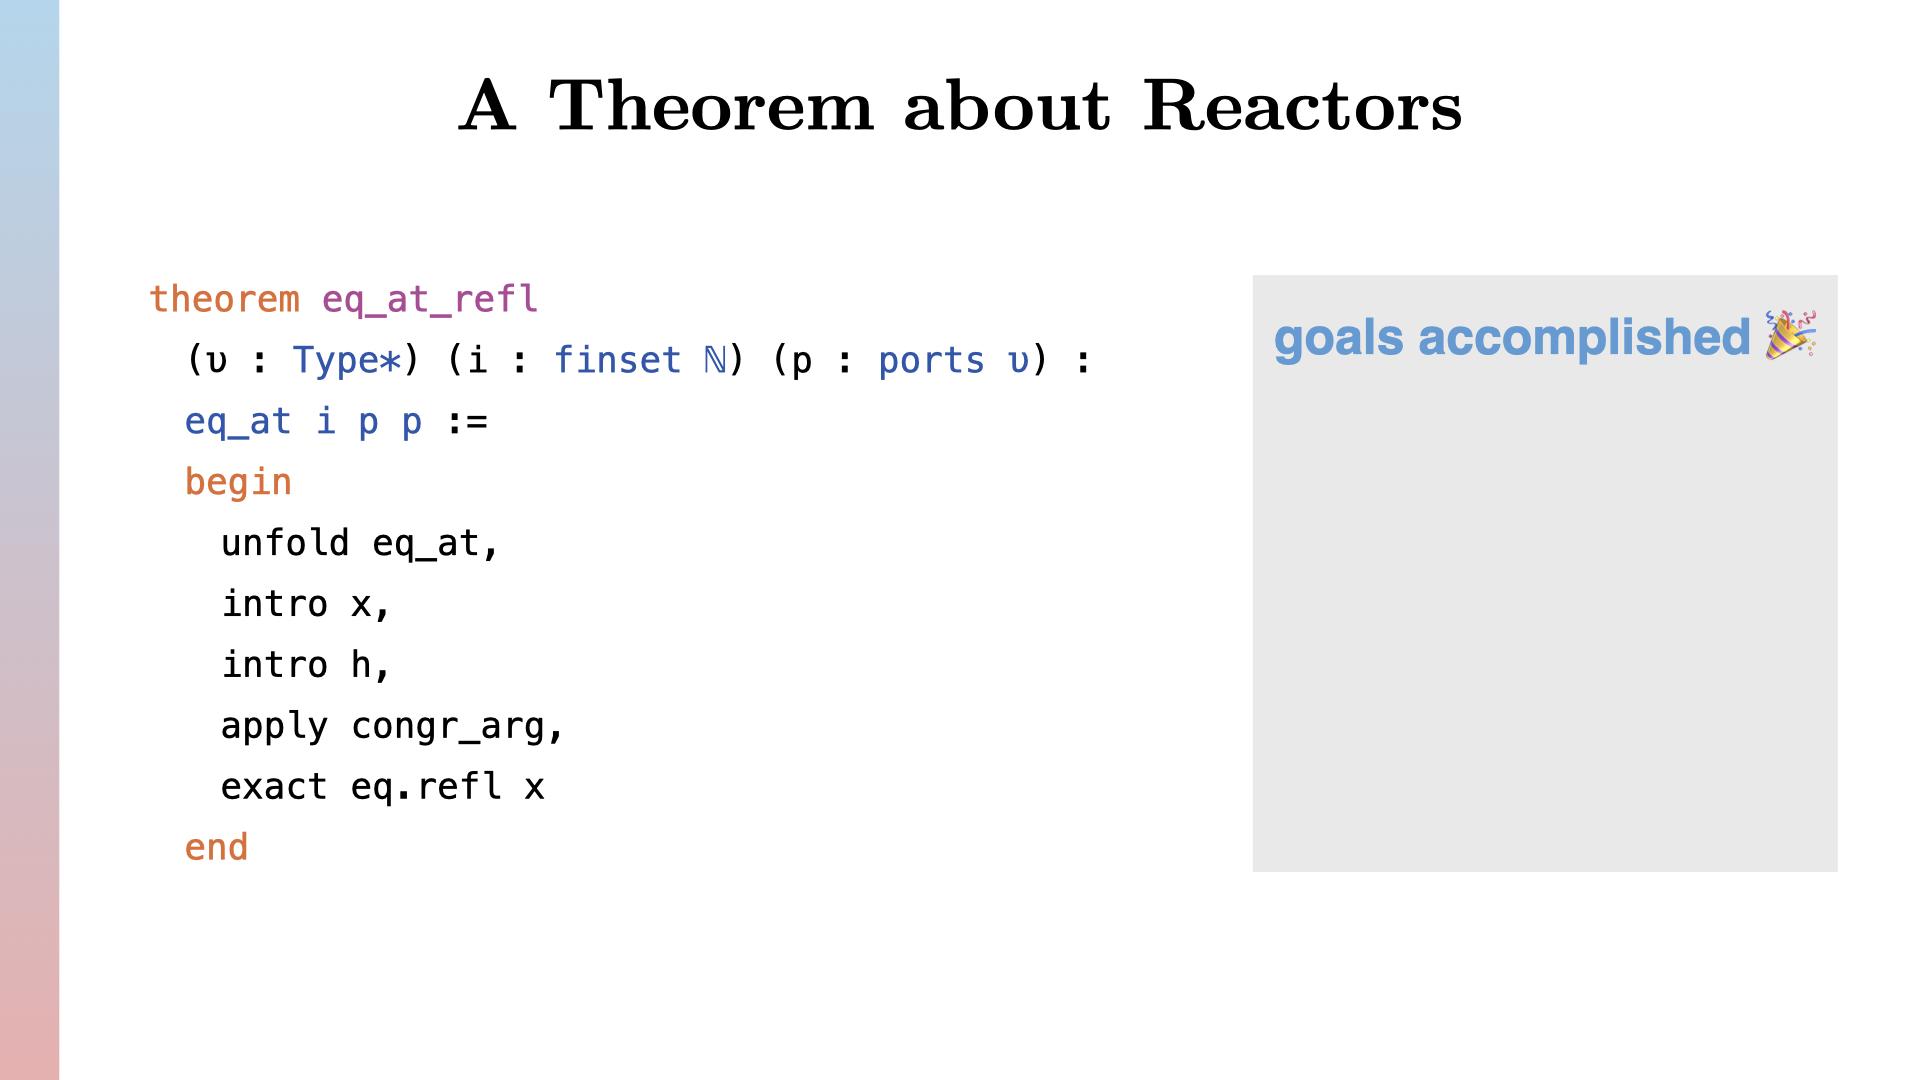
\includegraphics[width=\columnwidth]{Slides/Slide 18.jpeg}
\end{center}

Here you can see that the constructor for the equality type \lstinline{eq}
is called \lstinline{refl}. What you can also see is what can be a great
source of relief when proving complicated theorems: the message that
we've proven the theorem. As you get more skilled in Lean, you get
better at using tactic mode. For example, this theorem can actually be
proven in a single line. But when it comes down to it, tactics are
always just a mechanism for creating proof instance. Hence, proving
determinism for the Reactor model works exactly the same way. First, we
create a \lstinline{theorem}, where the type is precisely the statement
we're trying to prove.

\begin{center}
  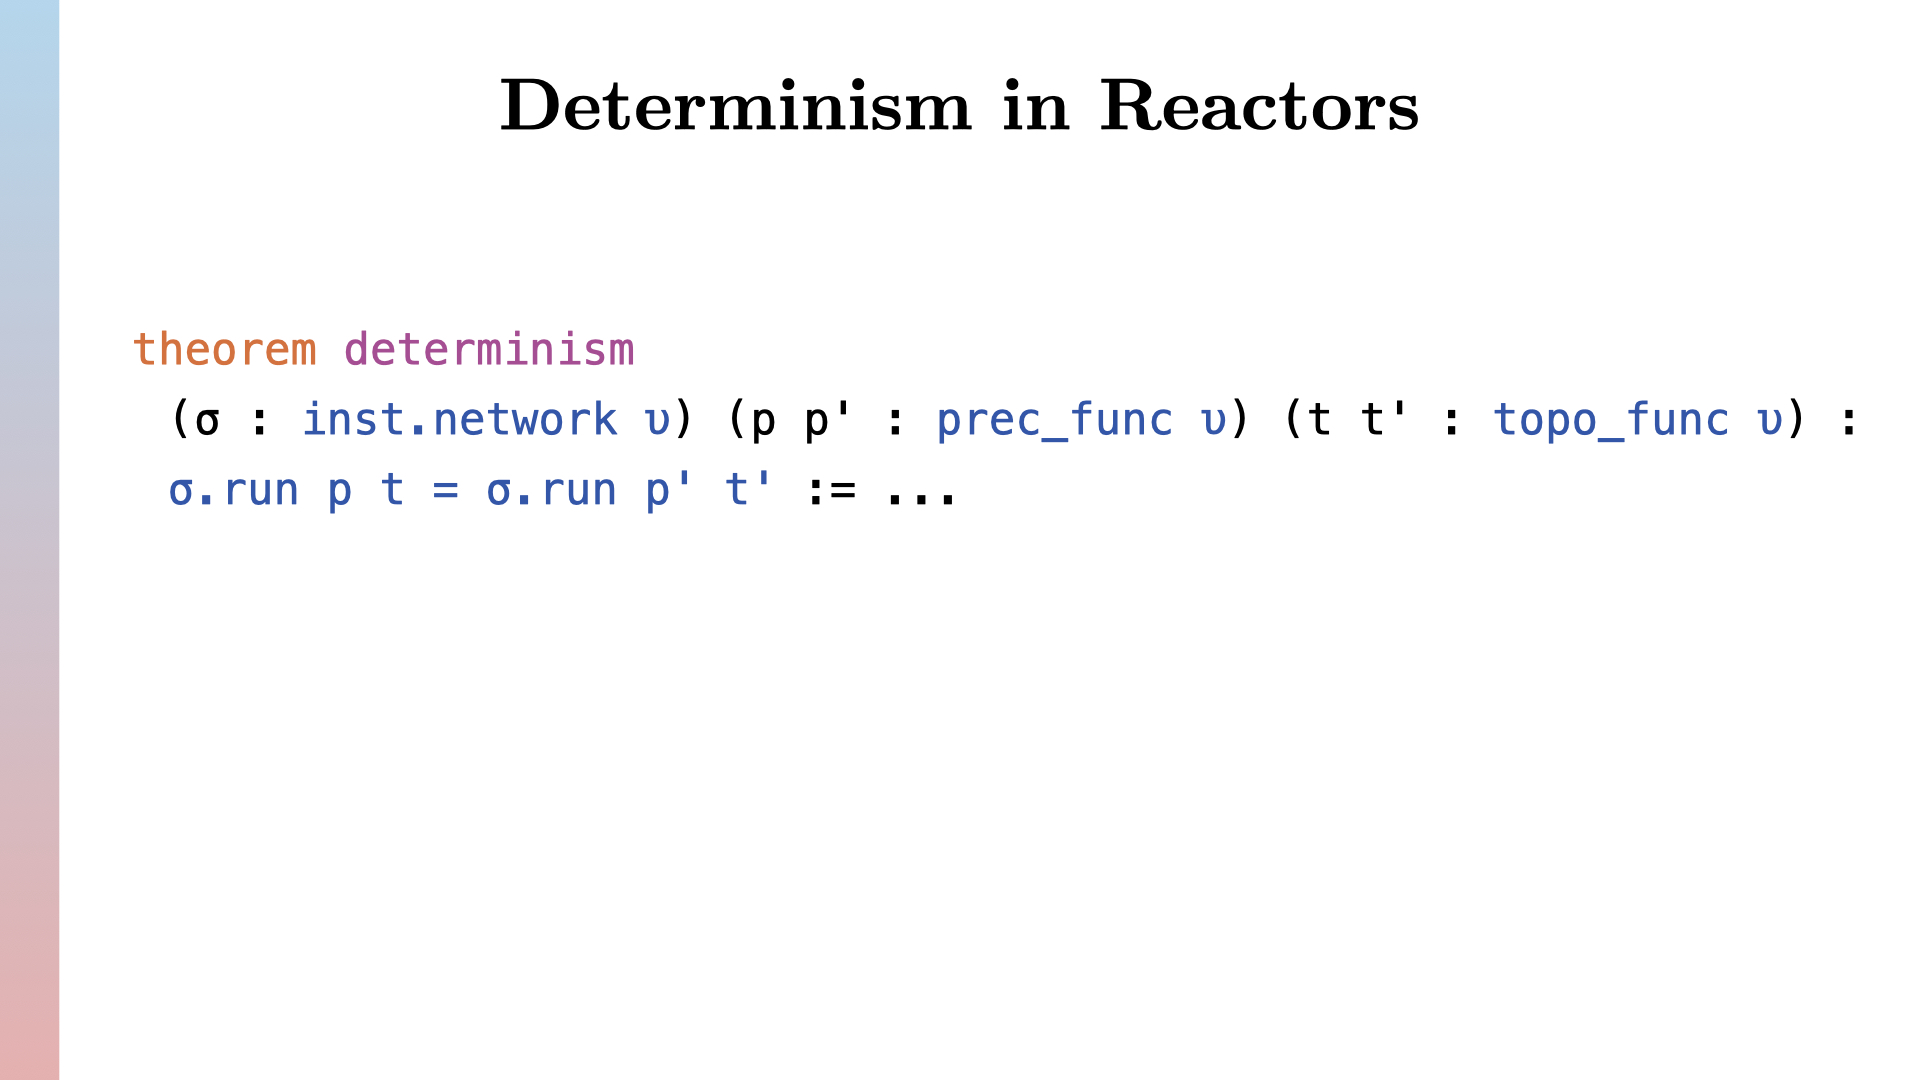
\includegraphics[width=\columnwidth]{Slides/Slide 19.jpeg}
\end{center}

In the case of \lstinline{determinism}, what we're proving is that running
a certain type of reactor network (\lstinline{inst.network}) always
produces the same outputs, independently of certain externalities
(\lstinline{prec_func} and \lstinline{topo_func}). And second, we prove the
statement using tactic mode. I won't show the proof of
\lstinline{determinism} here, because formalizing the small subset of the
Reactor model and proving \lstinline{determinism} actually took about 2000
lines of code --- but the approach was exactly what we've seen in the
previous slides. I'm guessing there might be some questions about this,
but for now we've reached the end of the slides. So for the main part of
this talk, we can consider all goals accomplished.

\begin{center}
  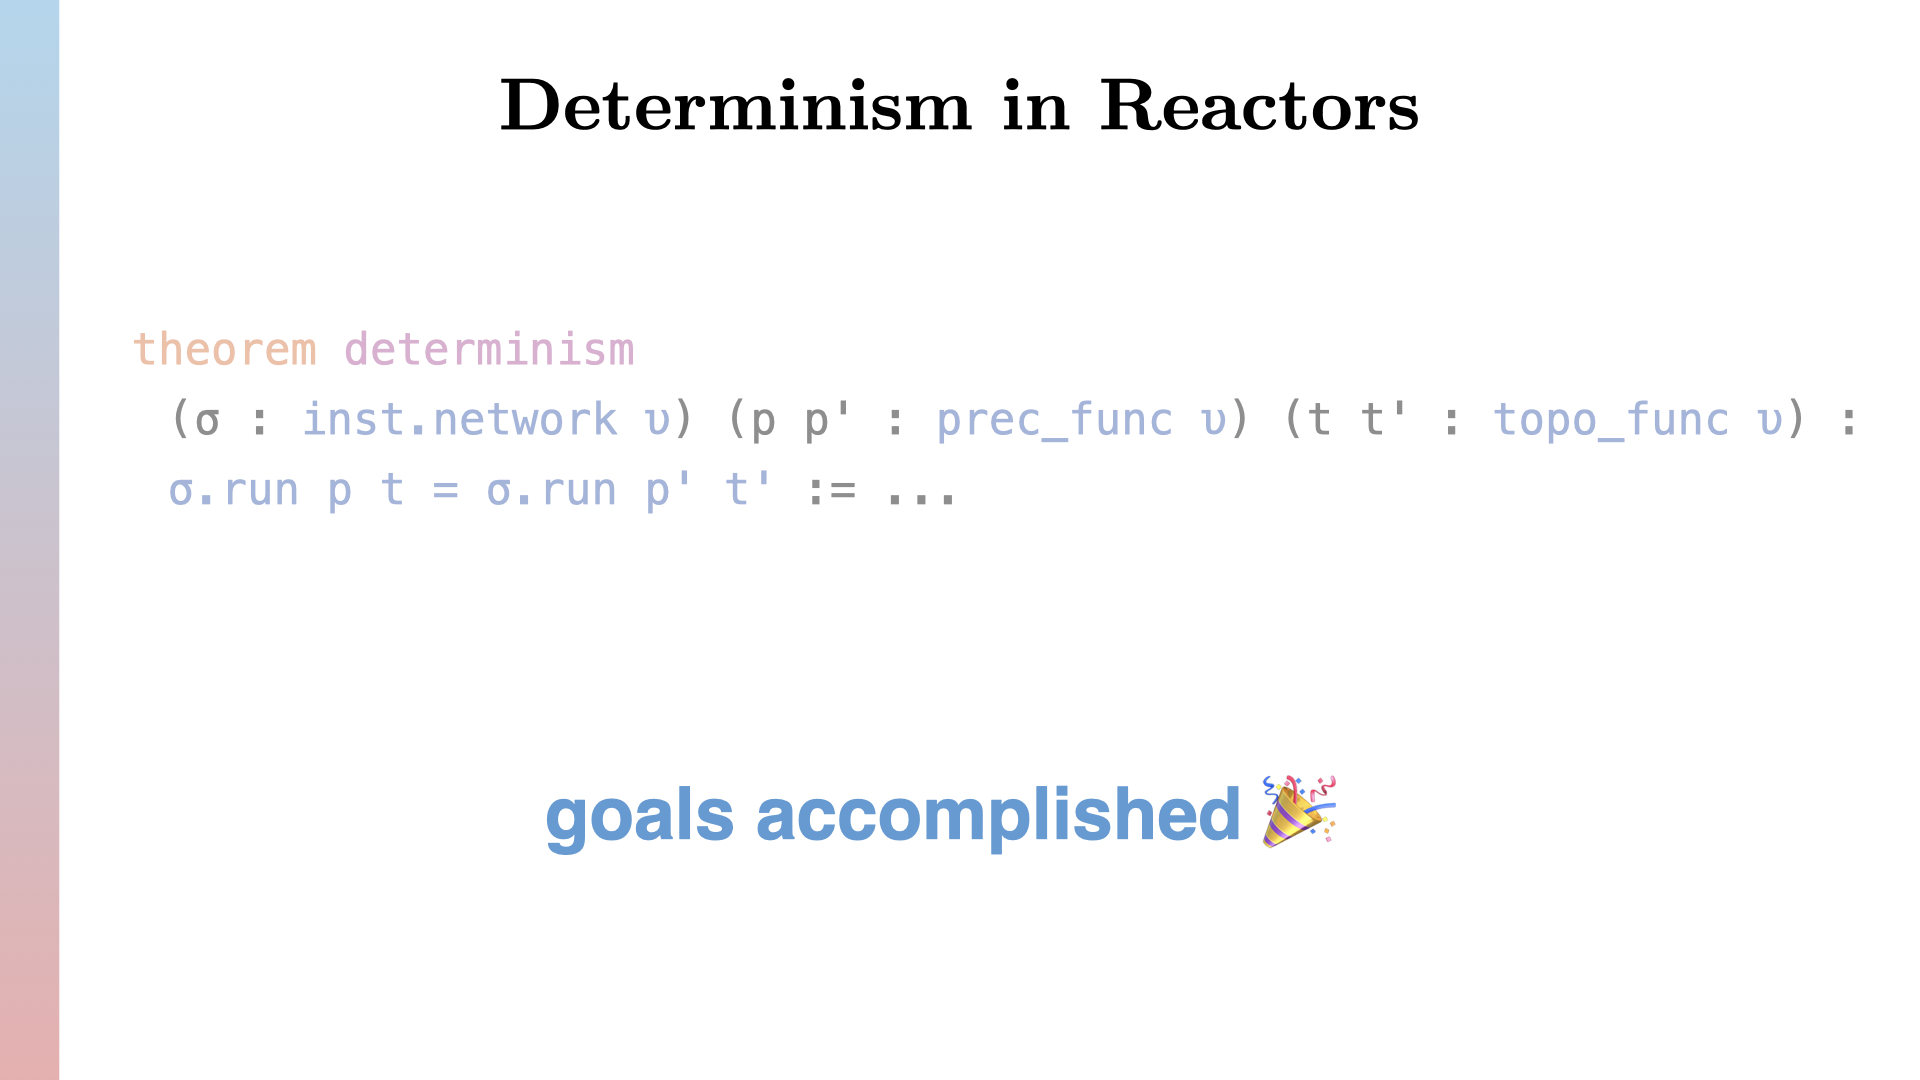
\includegraphics[width=\columnwidth]{Slides/Slide 20.jpeg}
\end{center}

\end{document}
